\section{Résultats}
Plusieurs scripts \emph{Python} ont été réalisés pour tester les différentes
méthodes de mesure. Cette section ne les détails pas, mais discutre des tests effectués
et de conclusions préliminaires.

\subsection{Mesure de débit de chute de neige} \label{snowfall}
Cette mesure doit permettre une information estimée de la chute de neige
actuelle. Idéalement, on devrait pouvoir estimer les précipitations de neige
en mm/h. Mais n'ayant pas encore reçu l'accès aux données de \emph{MeteoSwiss}
pour comparer nos mesures à des données fiables, une approche simplifiée a été
appliquée.\\
On récupère plusieurs vidéos qu'on trie selon 2 critères :
\begin{description}
    \item[Le moment de la journée] \hfill \\
    journée, nuit
    \item[La quantité visuelle de neige qui est en train de tomber] \hfill \\
    rien, petite chute de neige, neige, grosse chute de neige
\end{description}

\begin{figure}[H]
    \begin{subfigure}{.45\textwidth}
        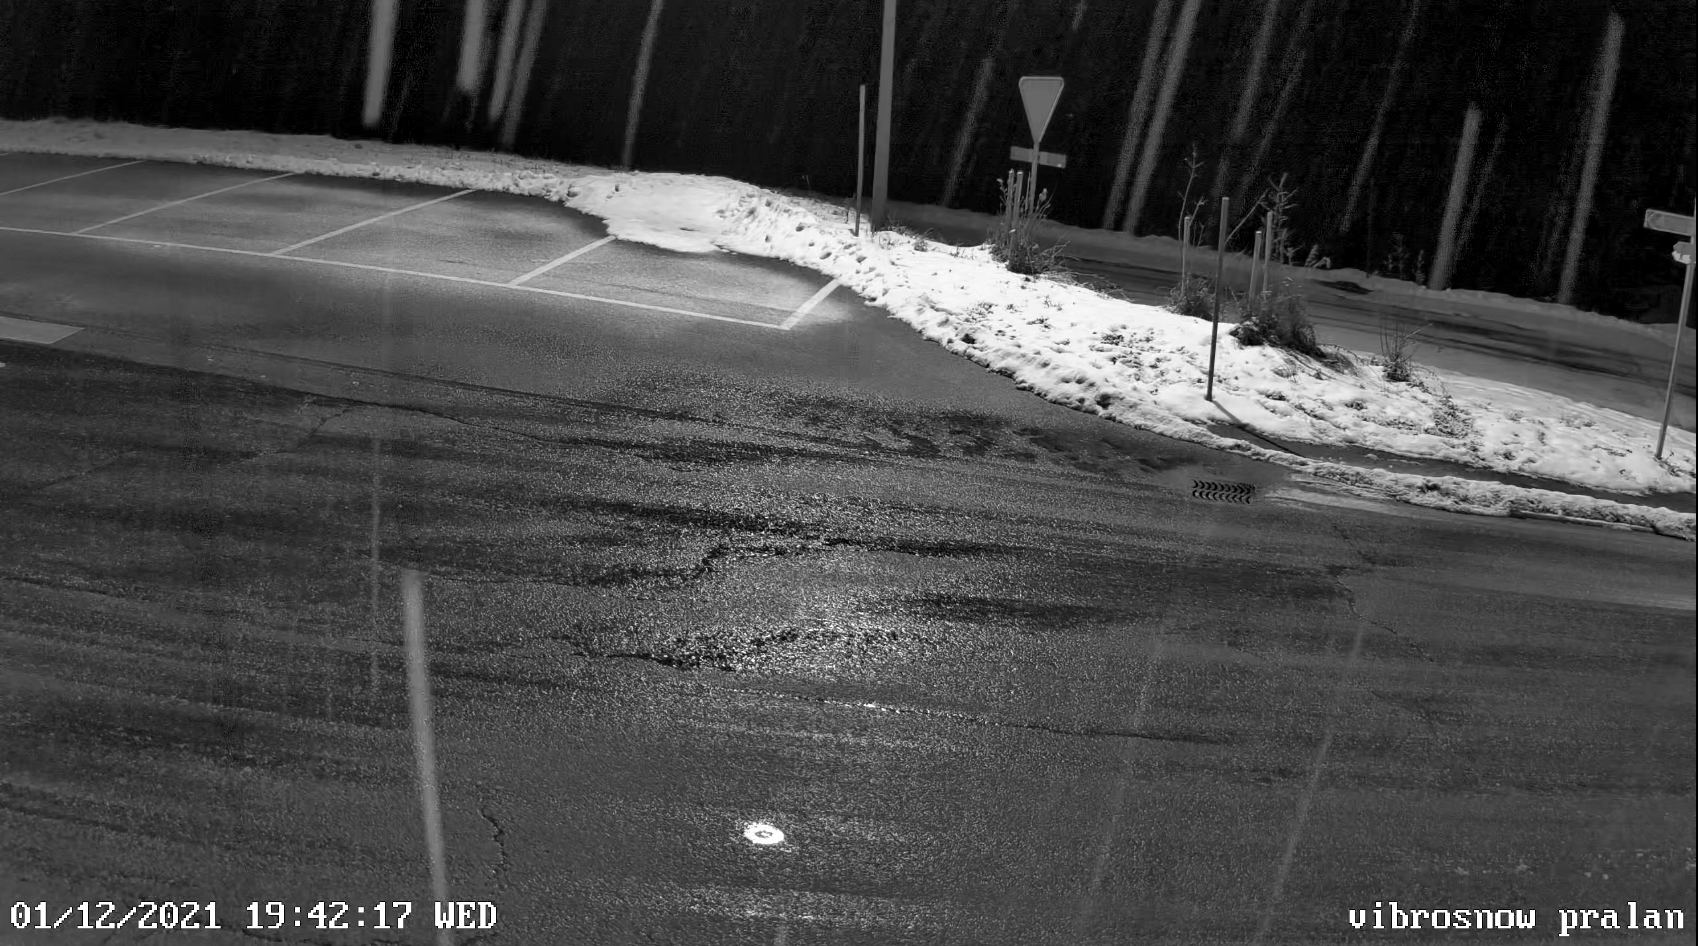
\includegraphics[width=\linewidth]{Images/computer_vision/snowfall/exemple_snow.PNG}
        \caption{Chute de neige (degré 2)}
        \label{fig:Snowfall_exempleSnow}
    \end{subfigure}
    \hfill
    \begin{subfigure}{.45\textwidth}
        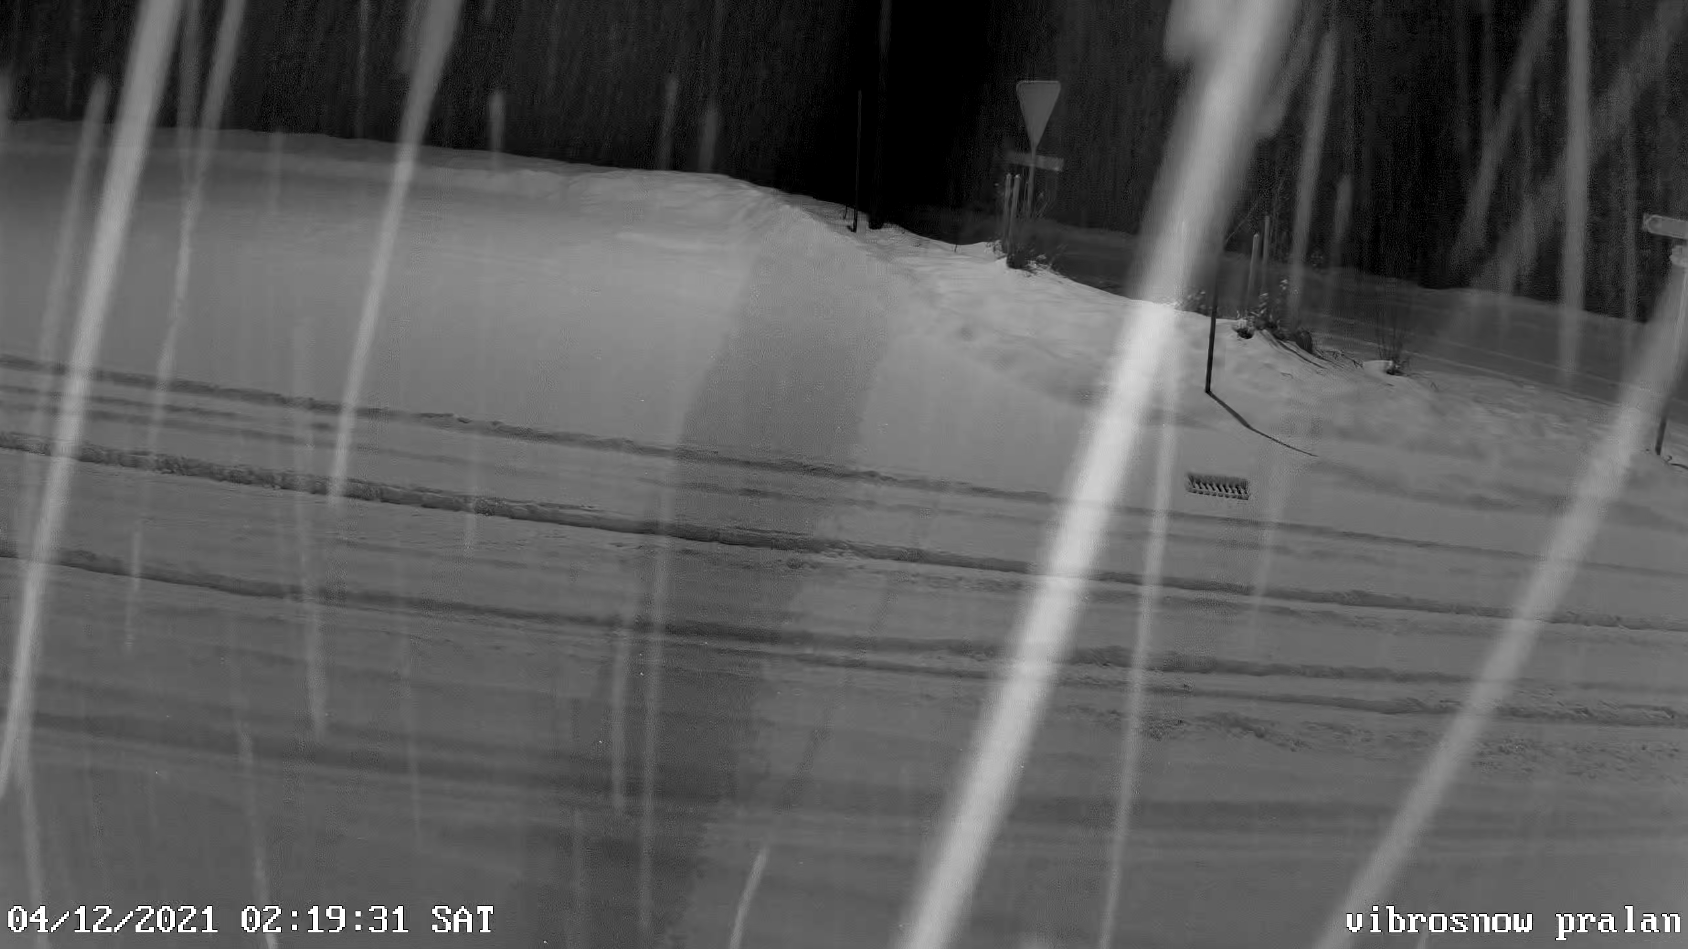
\includegraphics[width=\linewidth]{Images/computer_vision/snowfall/exemple_lotOfSnow.PNG}
        \caption{Grosse chute de neige (degré 3)}
        \label{fig:Snowfall_exempleLotOfSnow}
    \end{subfigure}
    \hfill
    \caption{Exemples de degré de chute de neige}
    \label{fig:Snowfall_exemples}
\end{figure}

Il est important de comparer des vidéos se passant durant la même période de la journée.
La luminosité peut grandement affecter le résultat de la mesure. La localisation
de la caméra (Ayent) ne permet pas de différencier significativement la matinée
de la journée et la soirée de la nuit. Il a donc été convenu de séparer uniquement
par jour/nuit.


\subsubsection{Résultats}
\begin{figure}[H]
    \begin{subfigure}{.45\textwidth}
        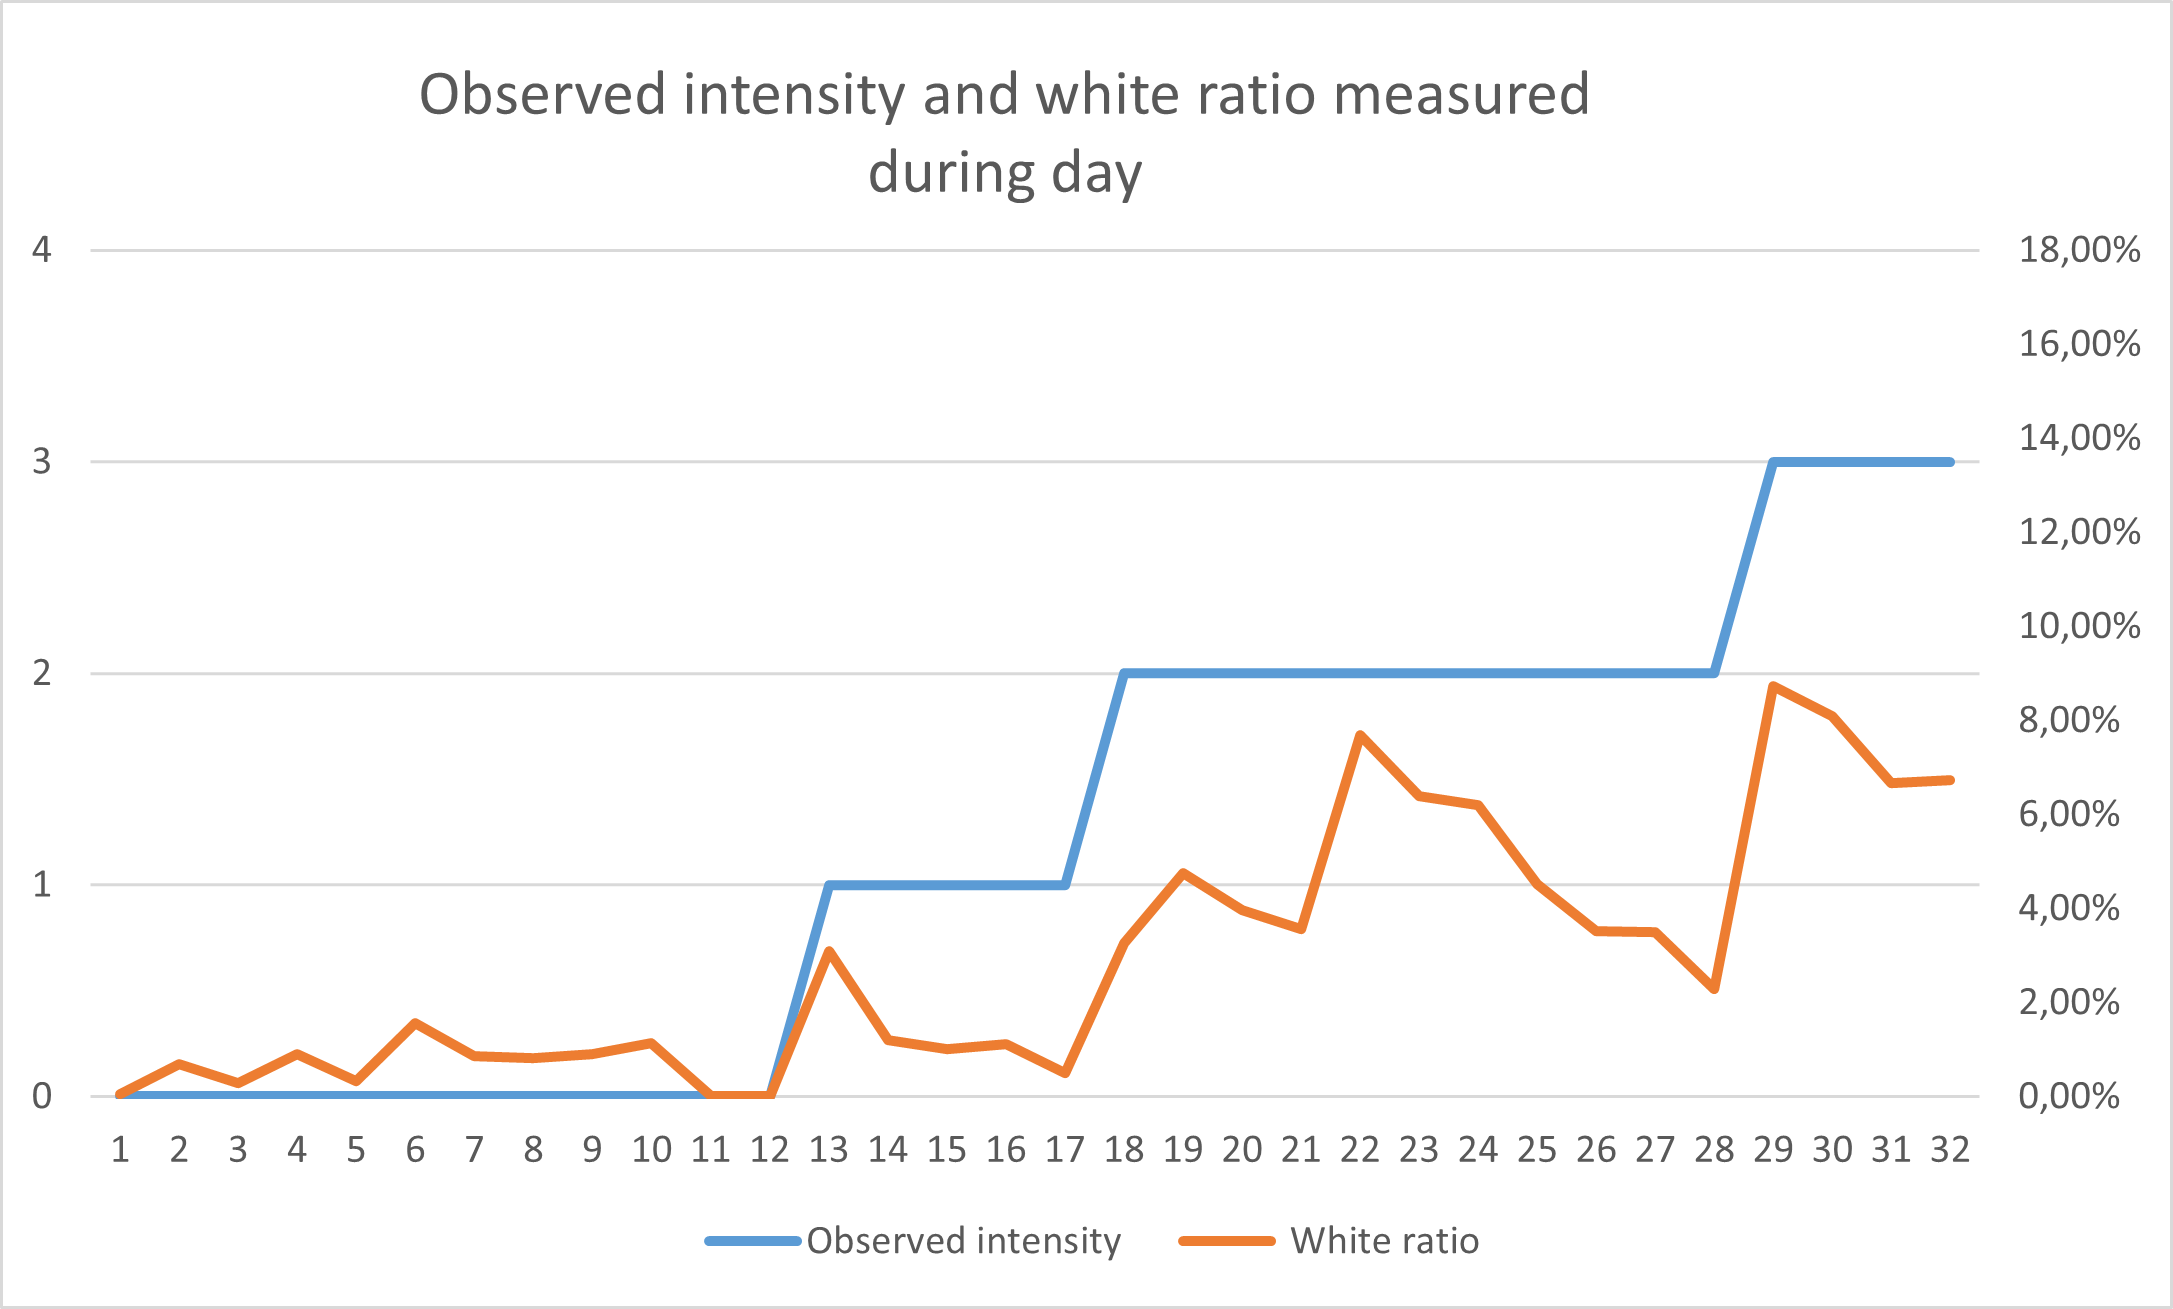
\includegraphics[width=\linewidth]{Images/computer_vision/snowfall/dayMes.png}
        \caption{Mesure durant la journée, en bleu la valeur jugée à l'oeil, en orange la valeur mesurée}
        \label{fig:Snowfall_dayMes}
    \end{subfigure}
    \hfill
    \begin{subfigure}{.45\textwidth}
        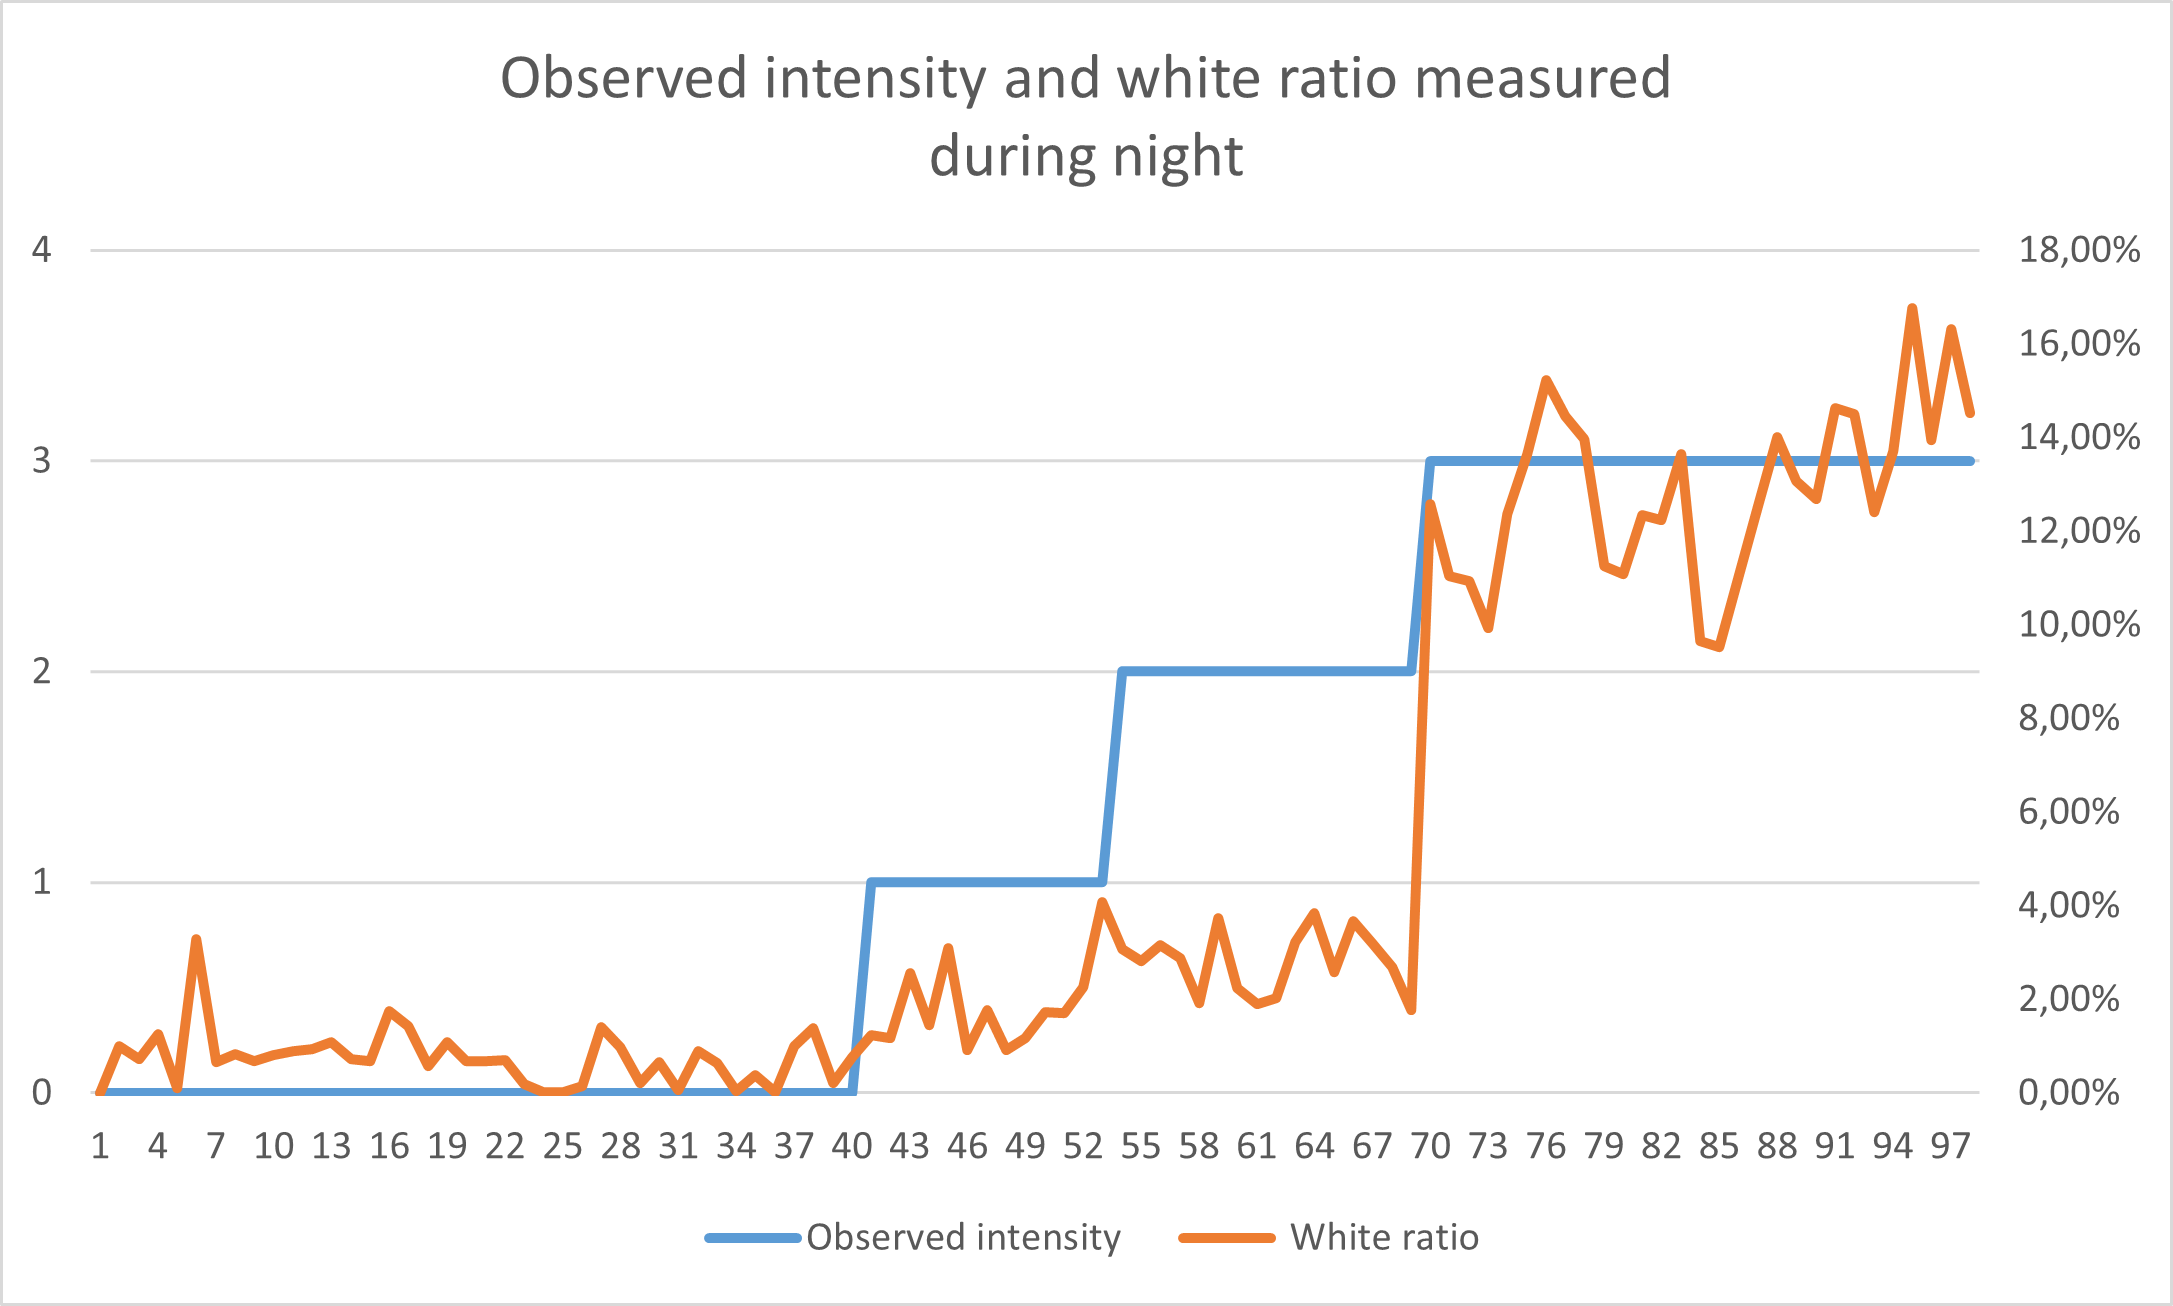
\includegraphics[width=\linewidth]{Images/computer_vision/snowfall/nightMes.png}
        \caption{Mesure durant la nuit, en bleu la valeur jugée à l'oeil, en orange la valeur mesurée}
        \label{fig:Snowfall_nightMes}
    \end{subfigure}
    \hfill
    \begin{subfigure}{.45\textwidth}
        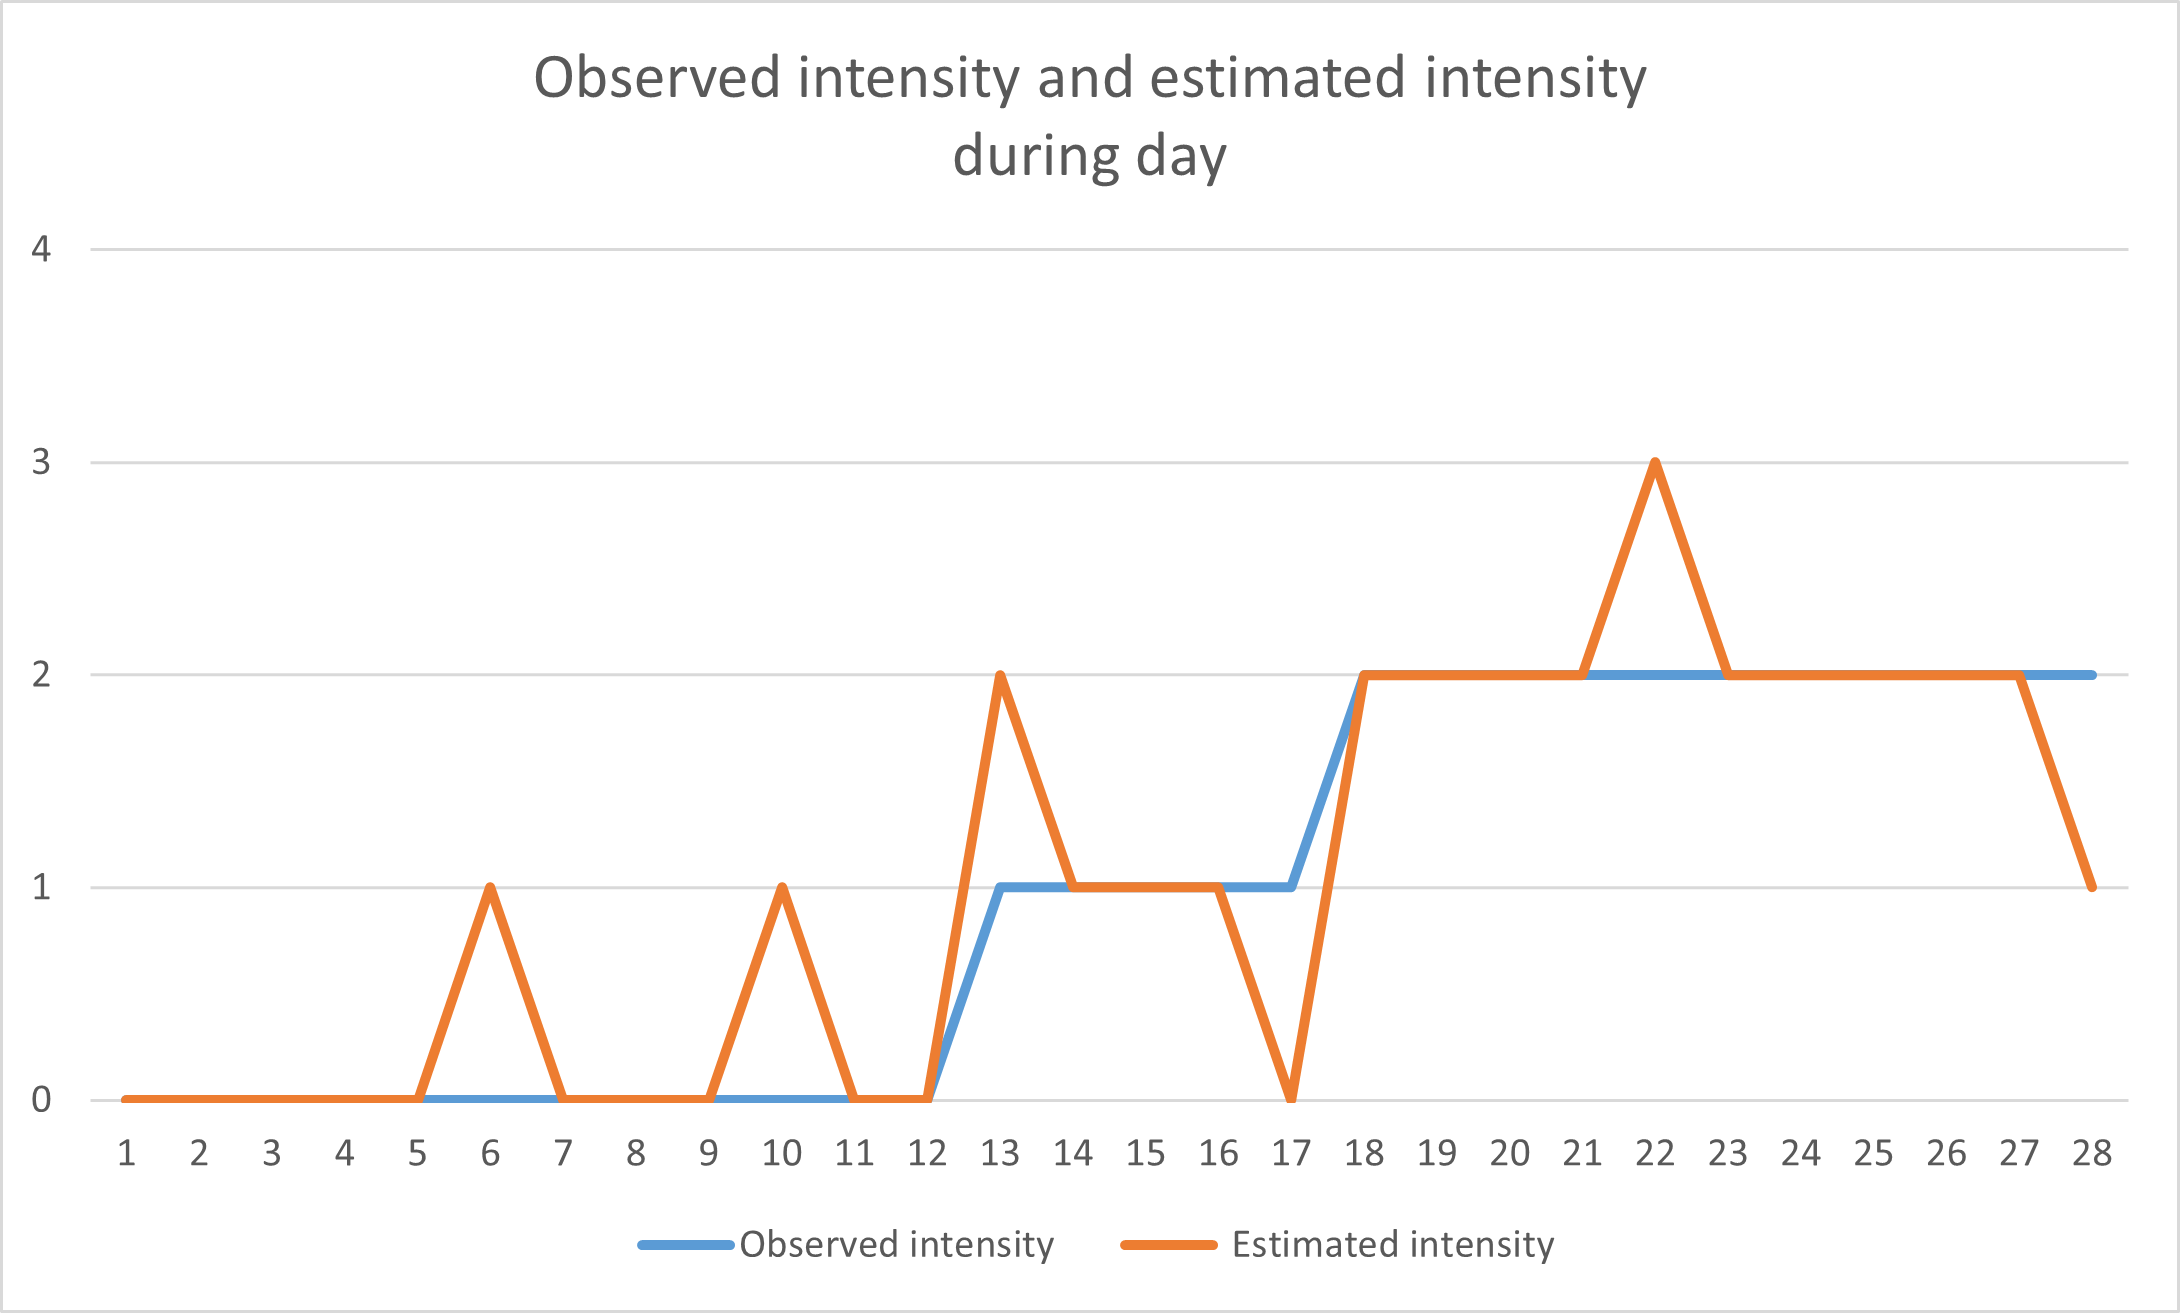
\includegraphics[width=\linewidth]{Images/computer_vision/snowfall/dayResults.png}
        \caption{Mesure durant la journée, en bleu la valeur jugée à l'oeil, en orange la valeur interprétée}
        \label{fig:Snowfall_dayResults}
    \end{subfigure}
    \hfill
    \begin{subfigure}{.45\textwidth}
        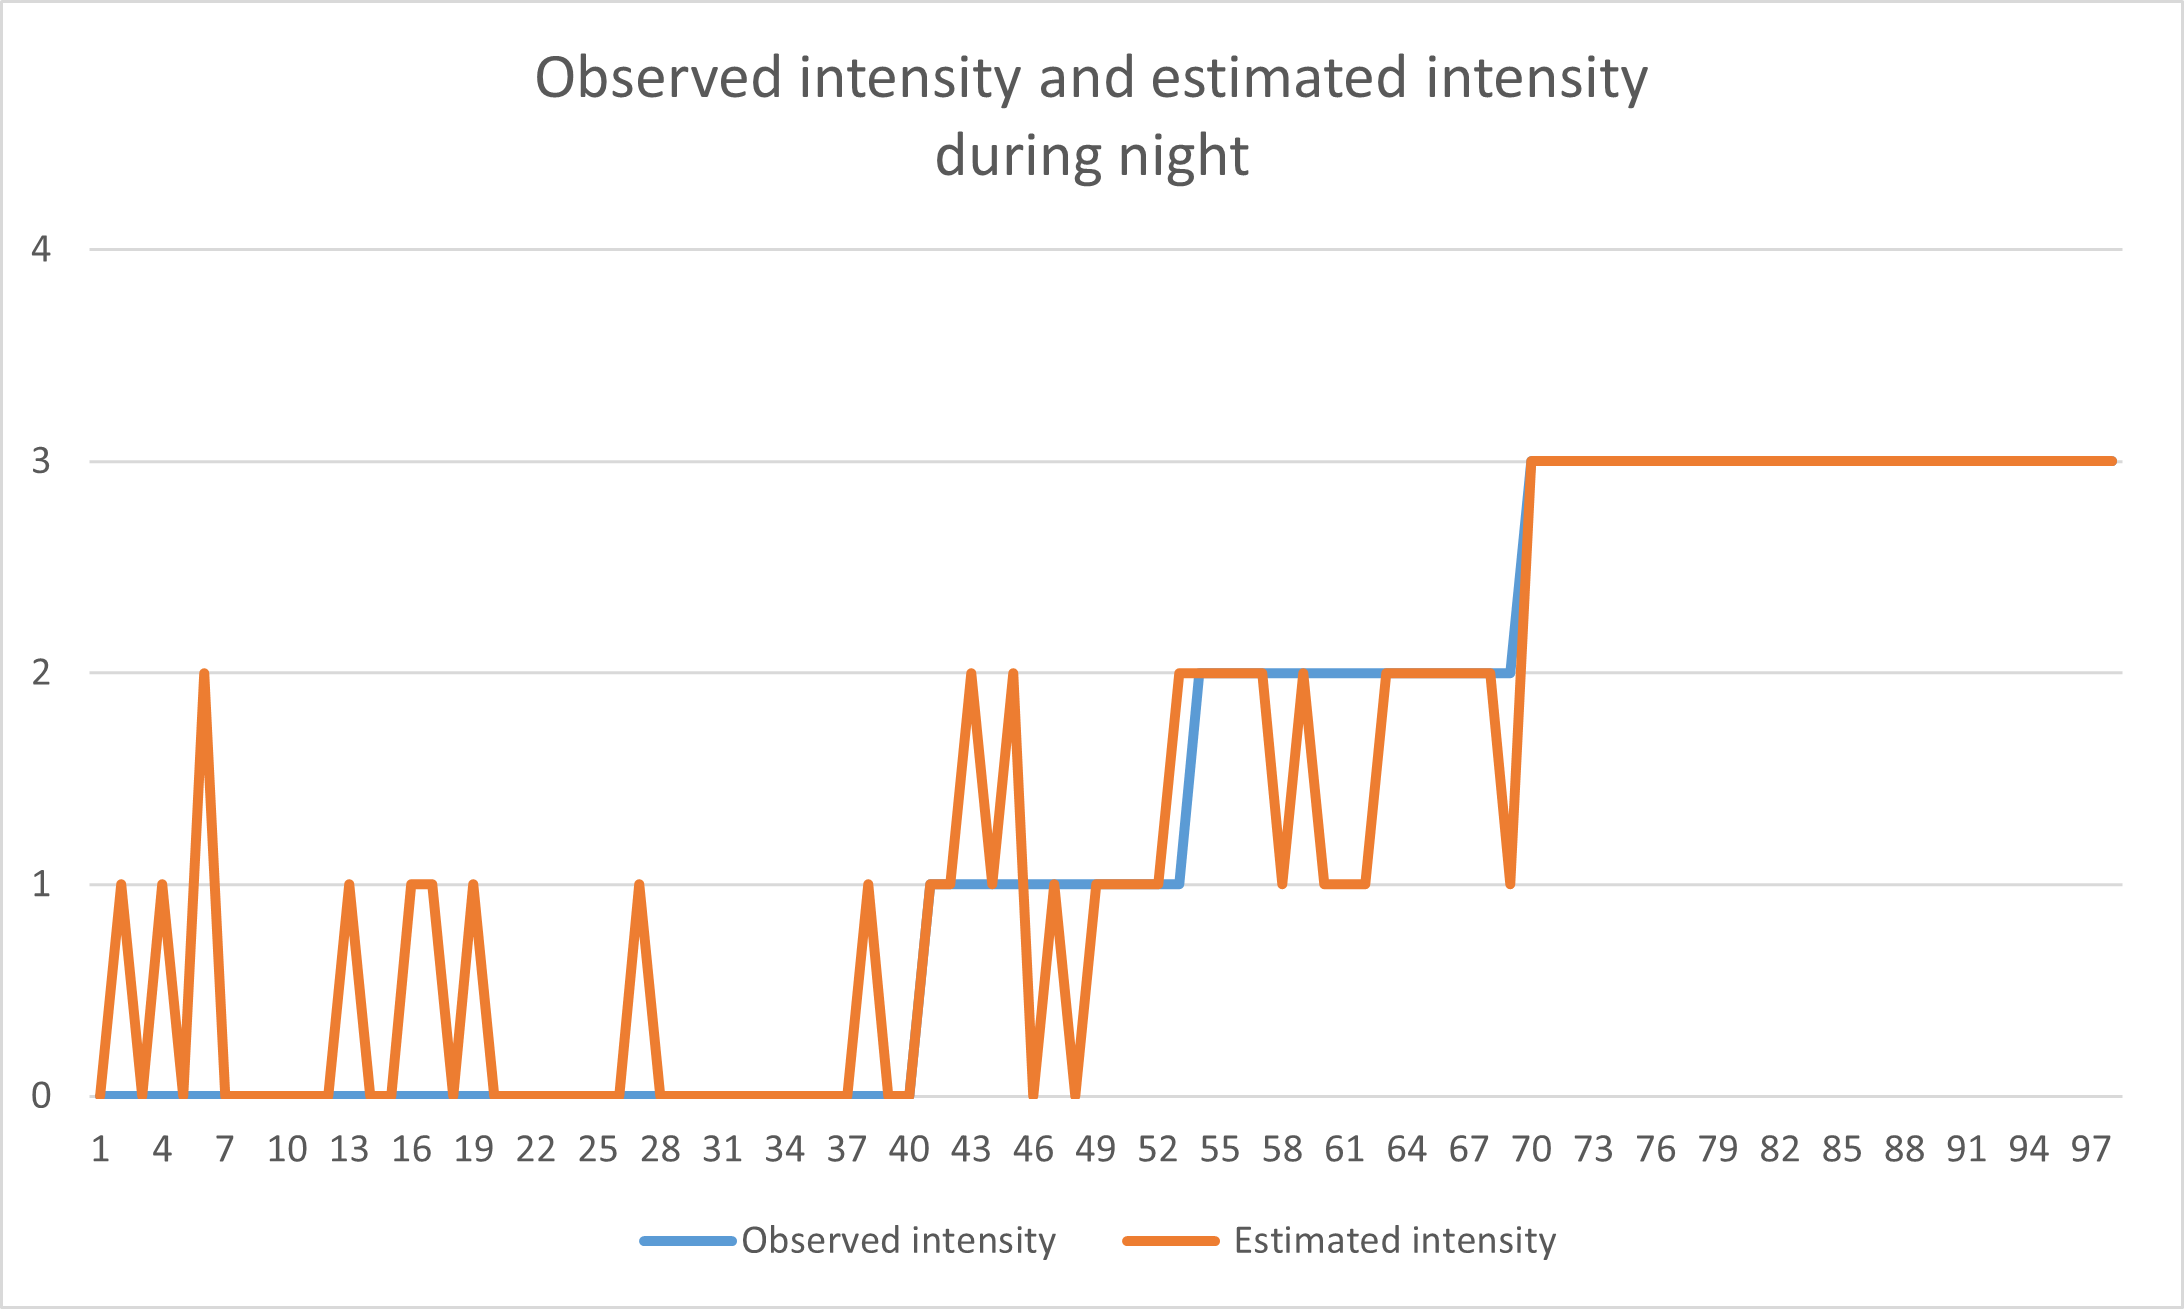
\includegraphics[width=\linewidth]{Images/computer_vision/snowfall/nightResults.png}
        \caption{Mesure durant la nuit, en bleu la valeur jugée à l'oeil, en orange la valeur interprétée}
        \label{fig:Snowfall_nightResults}
    \end{subfigure}
    \caption{Résultats de la mesure de débit de chute de neige \emph{(échelle : 0 pas de neige, 1 quelques flocons, 2 neige, 3 grosse chute de neige)}}
    \label{fig:Snowfall_results}
\end{figure}

\noindent
La précision de cette méthode est de $79.2\%$ sur cet échantillon. Les erreurs au degré 0 sont entièrement dues aux véhicules qui passent.
En effet la caméra n'enregistre uniquement lorsqu'elle détecte un mouvement.

\subsubsection{Conclusion préliminaire}
Cette méthode est suffisamment précise pour détecter le débit de neige. Cependant il faudrait
ajouter une méthode évitant de prendre la mesure lorsqu'un véhicule passe.
Les degrés mesurés peuvent être \emph{fine tuned} en expérimentant avec plus de vidéos et des données météos fiables.\newpage

\subsection{Détection de route enneigée}
Le but de cette mesure est de fournir, a minima, si oui ou non la route
est enneigée. Idéalement elle devrait pouvoir différencier plusieurs degrés
d'enneigement de la route. \\
Pour réaliser les mesures, on récupère plusieurs vidéos qu'on trie ainsi :
\begin{description}
    \item[Le moment de la journée] \hfill \\
    journée, nuit 
    \item[L'état de la route] \hfill \\
    déneigée, partiellement enneigée, complêtement enneigée 
\end{description}

\begin{figure}[H]
    \begin{subfigure}{.45\textwidth}
        \includegraphics[width=\linewidth]{Images/computer_vision/snowOnRoad/example_1.PNG}
        \caption{Route partiellement couverte (degré 1)}
        \label{fig:SnowOnRoad_exemplePartial}
    \end{subfigure}
    \hfill
    \begin{subfigure}{.45\textwidth}
        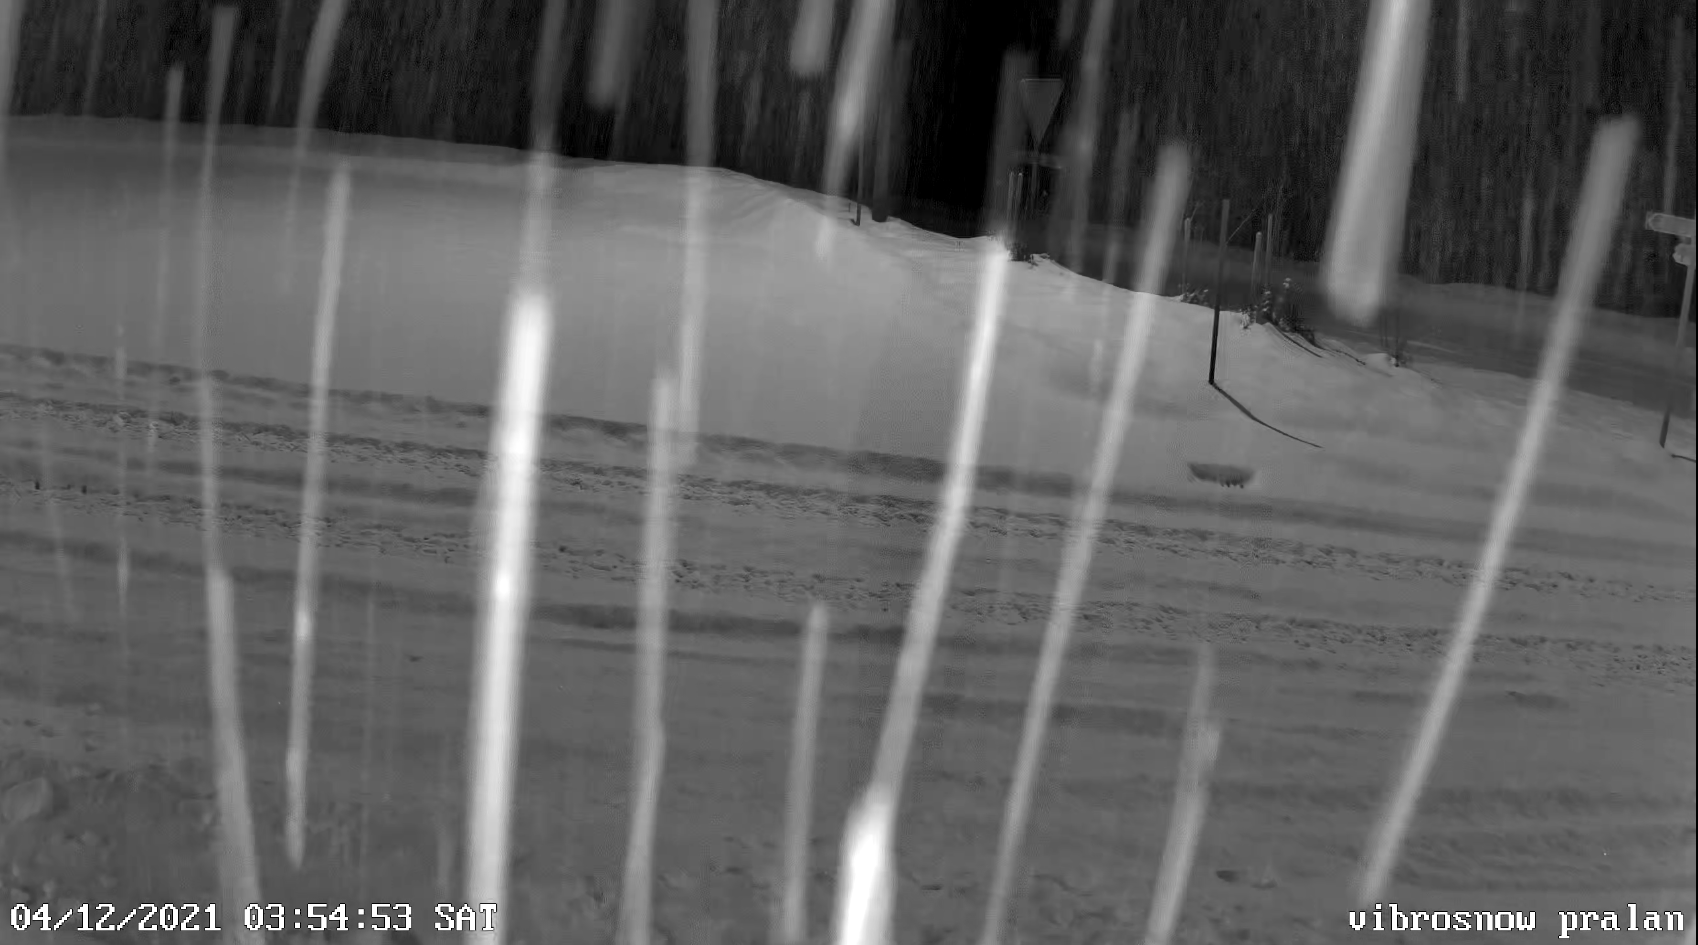
\includegraphics[width=\linewidth]{Images/computer_vision/snowOnRoad/example_2.PNG}
        \caption{Route entièrement couverte (degré 2)}
        \label{fig:SnowOnRoad_exempleFully}
    \end{subfigure}
    \hfill
    \caption{Exemples de degré d'état de la route}
    \label{fig:SnowOnRoad_exemples}
\end{figure}

La séparation jour/nuit est importante pour cette mesure. Si la route est encore humide,
la lumière du soleil peut si réfléchir et fausser la mesure. C'est pourquoi des valeurs de seuils différentes
ont été utilisées ici ($80/255$ pour la nuit et $120/255$ pour le jour).\\
Chaque vidéo sans chute de neige avec une route déneigée peut servir de 
référence pour différencier une route déneigée d'une route enneigée.\\
Dans l'idéal, on devrait aussi pouvoir les trier selon la quantité de chute
de neige, mais n'ayant pas suffisamment de vidéos pour réaliser ce tri, on devra
se contenter de cette méthode.\\
Les deux méthodes de mesure citées au point \ref{snowOnRoad} vont être mises
à l'épreuve pour déterminer laquelle est la plus pertinente pour ce projet.

\subsubsection{Sans traitement}
\begin{figure}[H]
    \begin{subfigure}{.45\textwidth}
        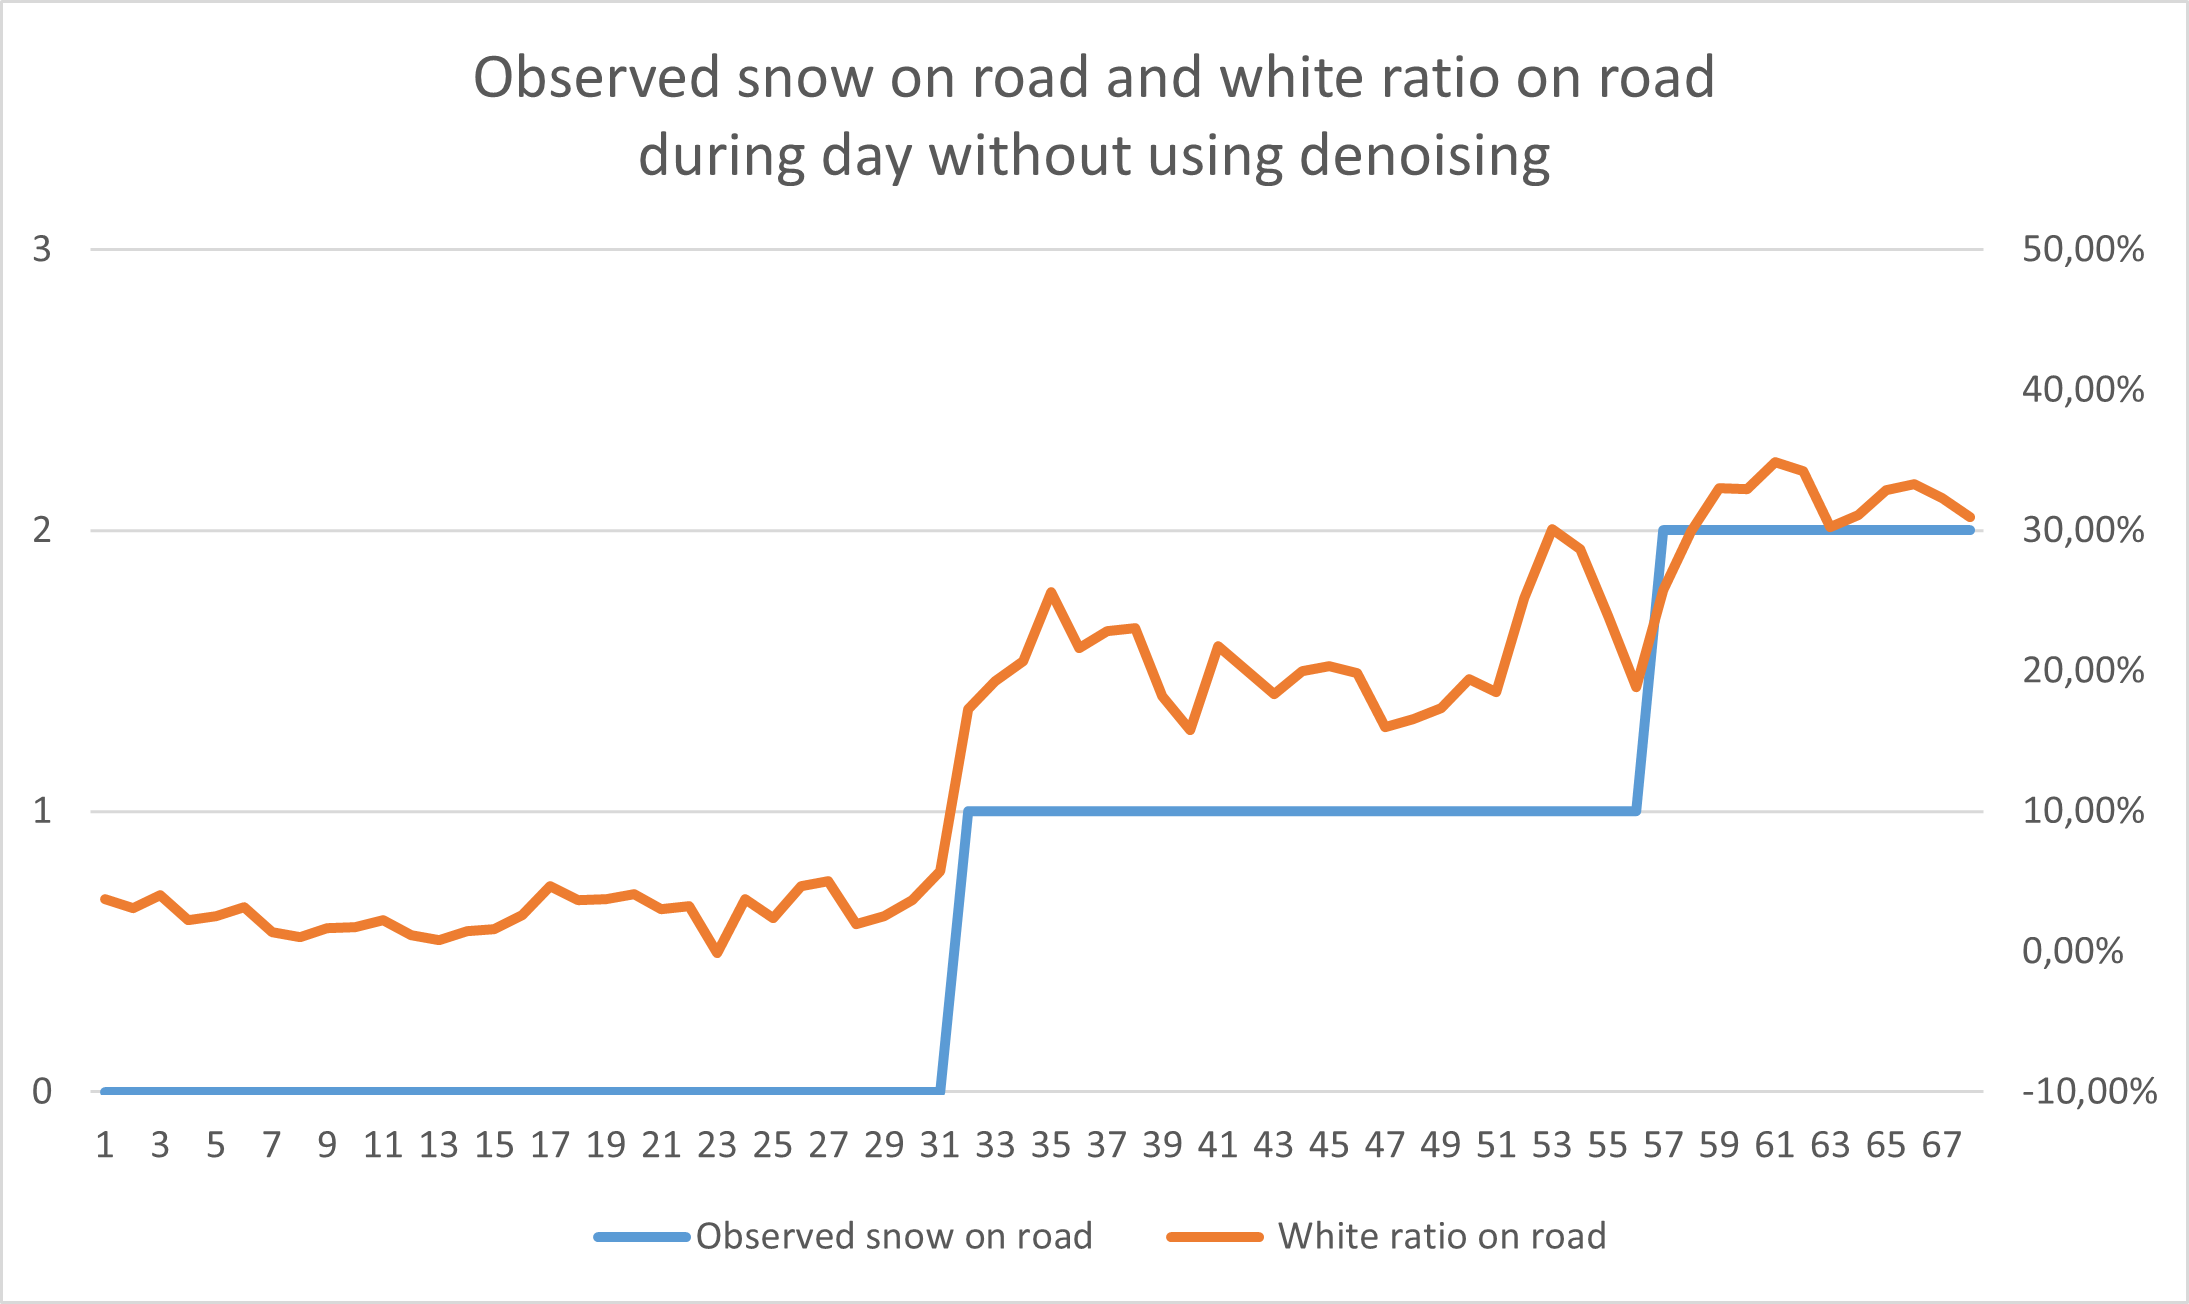
\includegraphics[width=\linewidth]{Images/computer_vision/snowOnRoad/dayMes_noise.png}
        \caption{Mesure durant la journée, en bleu la valeur jugée à l'oeil, en orange la valeur mesurée}
        \label{fig:SnowOnRoad_noise_dayMes}
    \end{subfigure}
    \hfill
    \begin{subfigure}{.45\textwidth}
        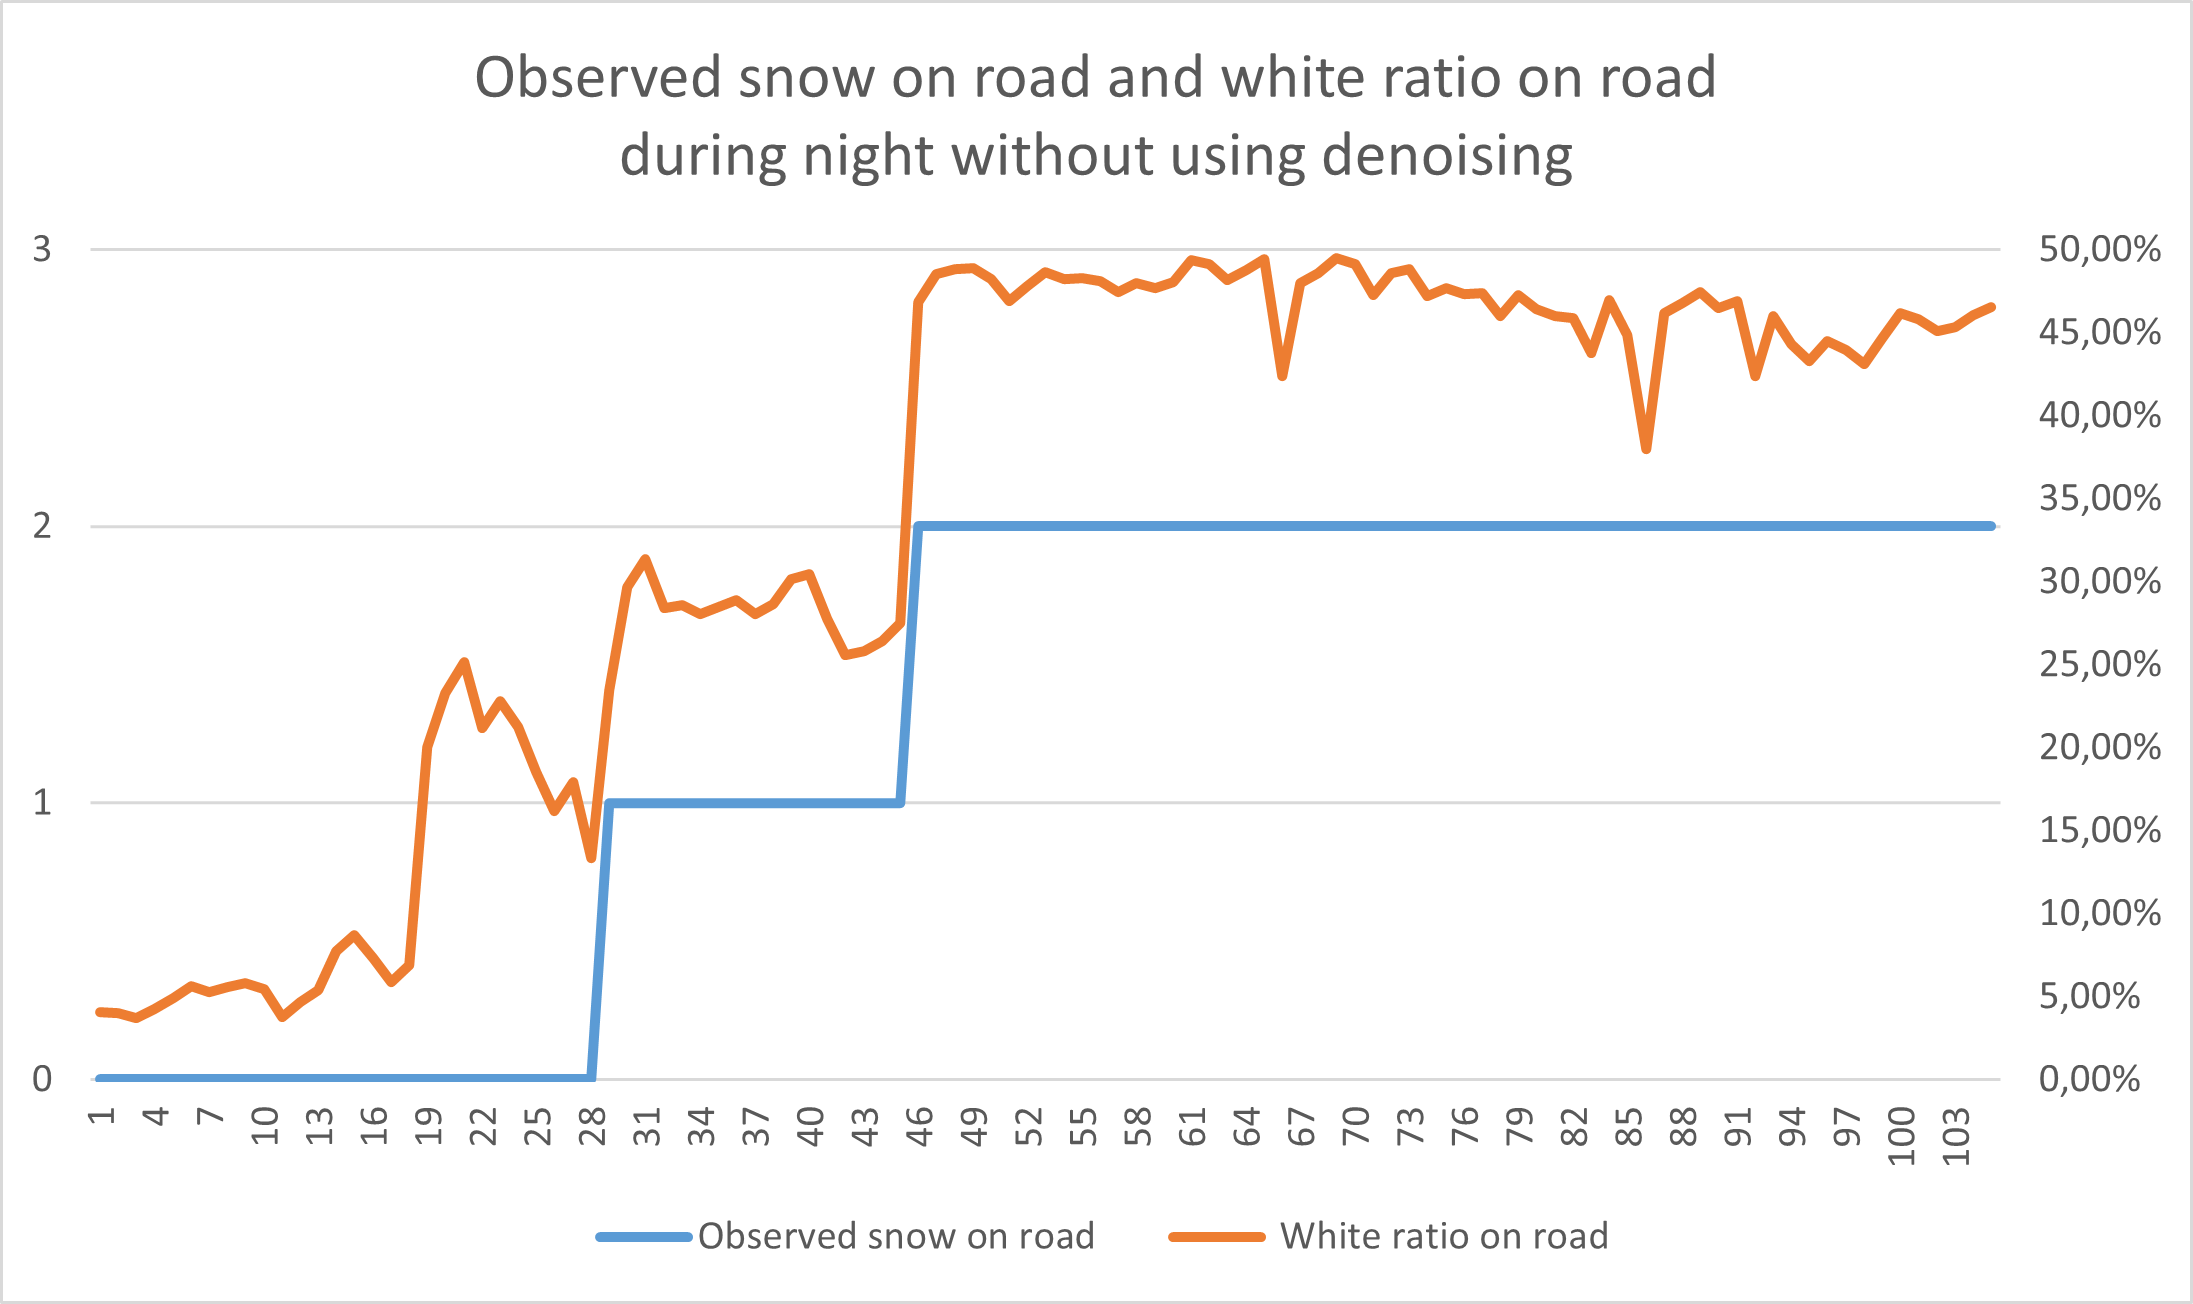
\includegraphics[width=\linewidth]{Images/computer_vision/snowOnRoad/nightMes_noise.png}
        \caption{Mesure durant la nuit, en bleu la valeur jugée à l'oeil, en orange la valeur mesurée}
        \label{fig:SnowOnRoad_noise_nightMes}
    \end{subfigure}
    \hfill
    \begin{subfigure}{.45\textwidth}
        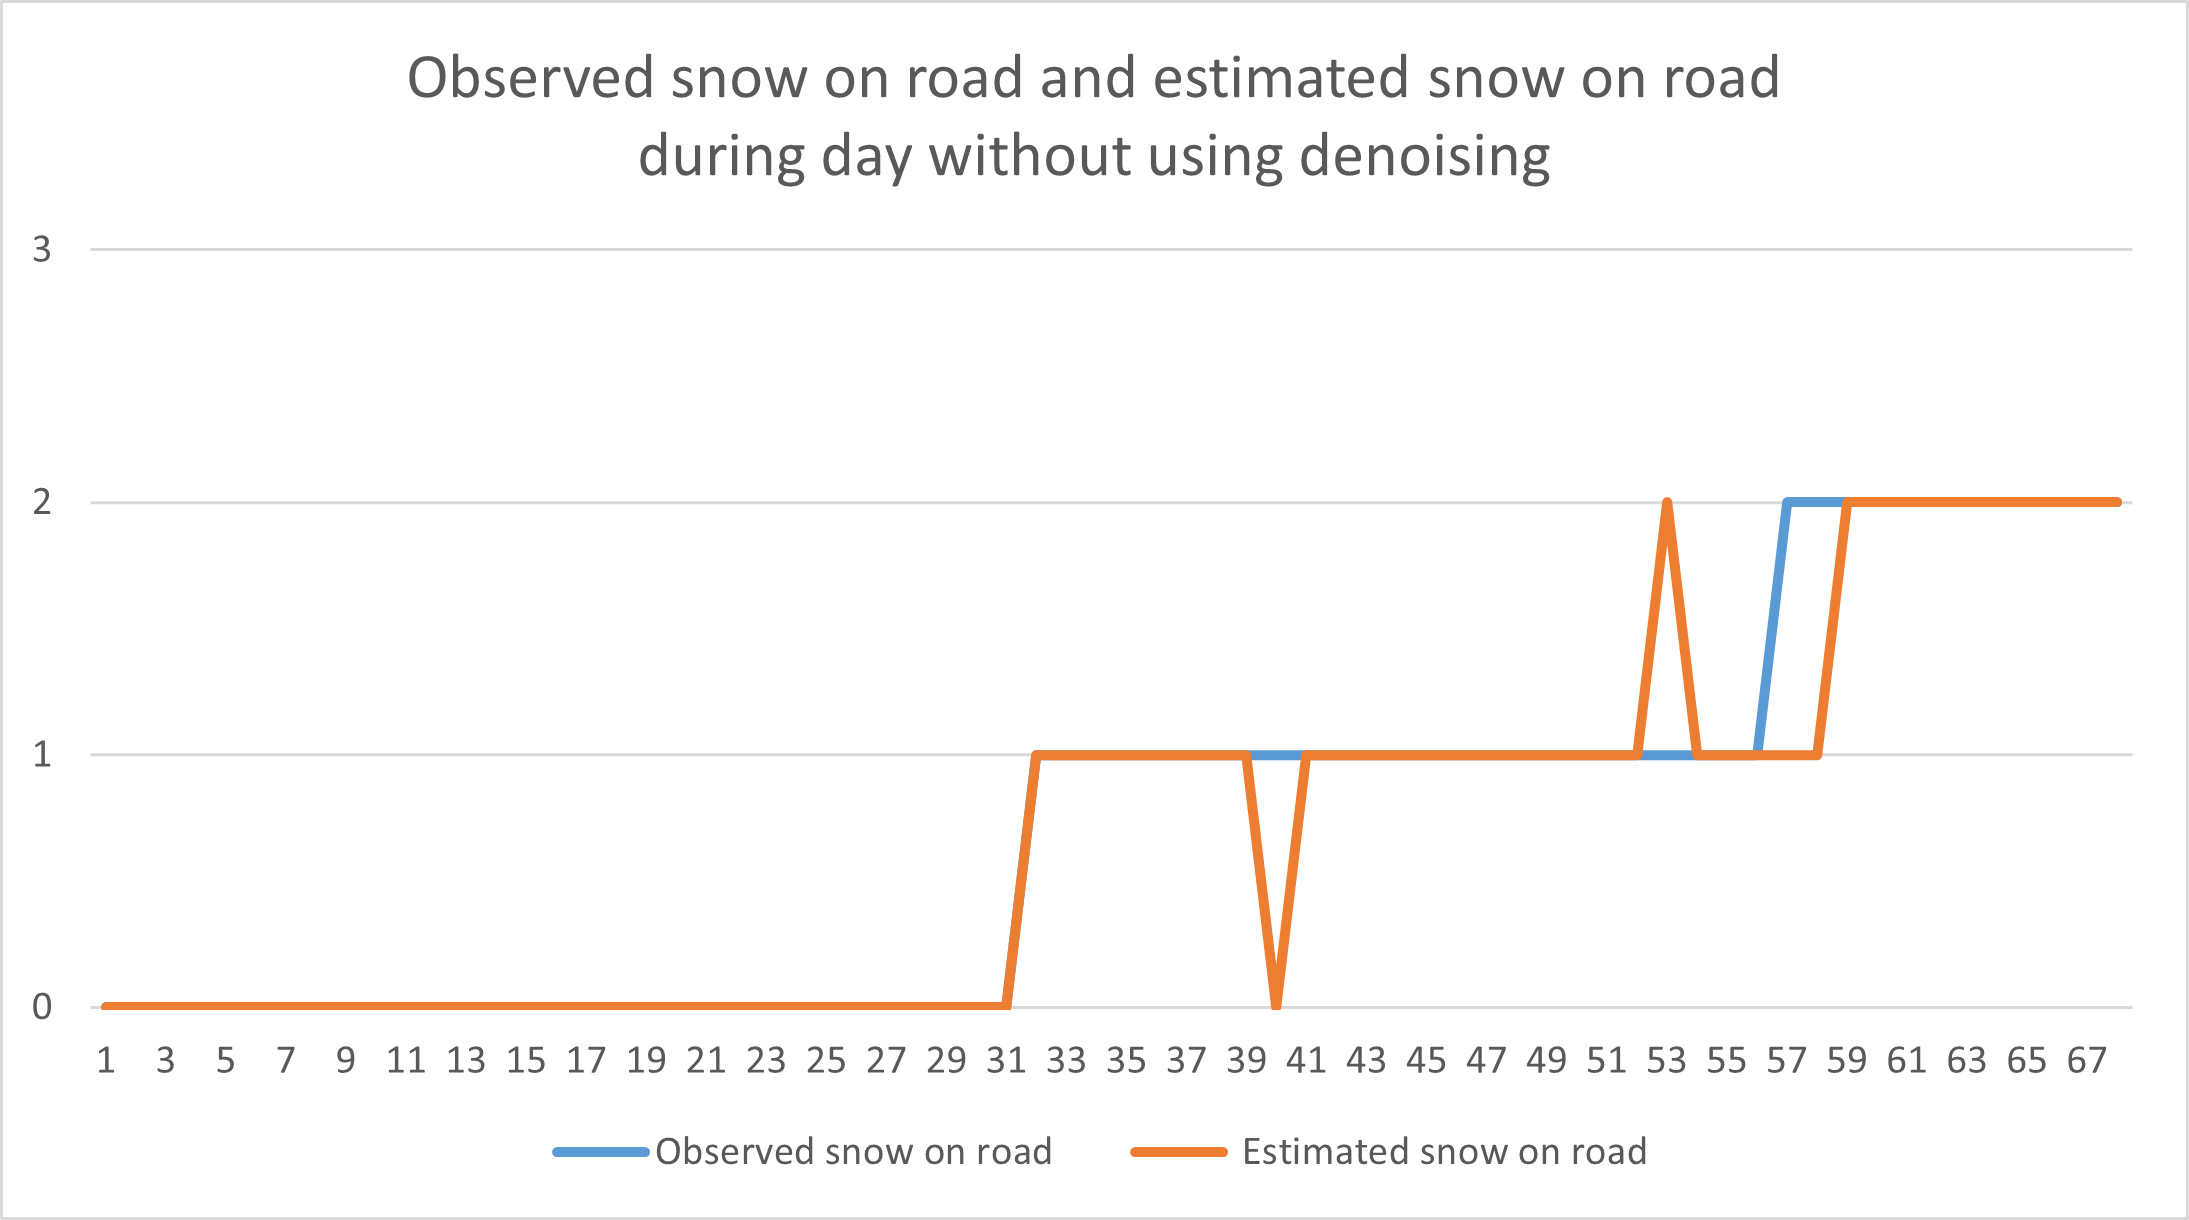
\includegraphics[width=\linewidth]{Images/computer_vision/snowOnRoad/dayResults_noise.png}
        \caption{Mesure durant la journée, en bleu la valeur jugée à l'oeil, en orange la valeur interprétée}
        \label{fig:SnowOnRoad_noise_dayResults}
    \end{subfigure}
    \hfill
    \begin{subfigure}{.45\textwidth}
        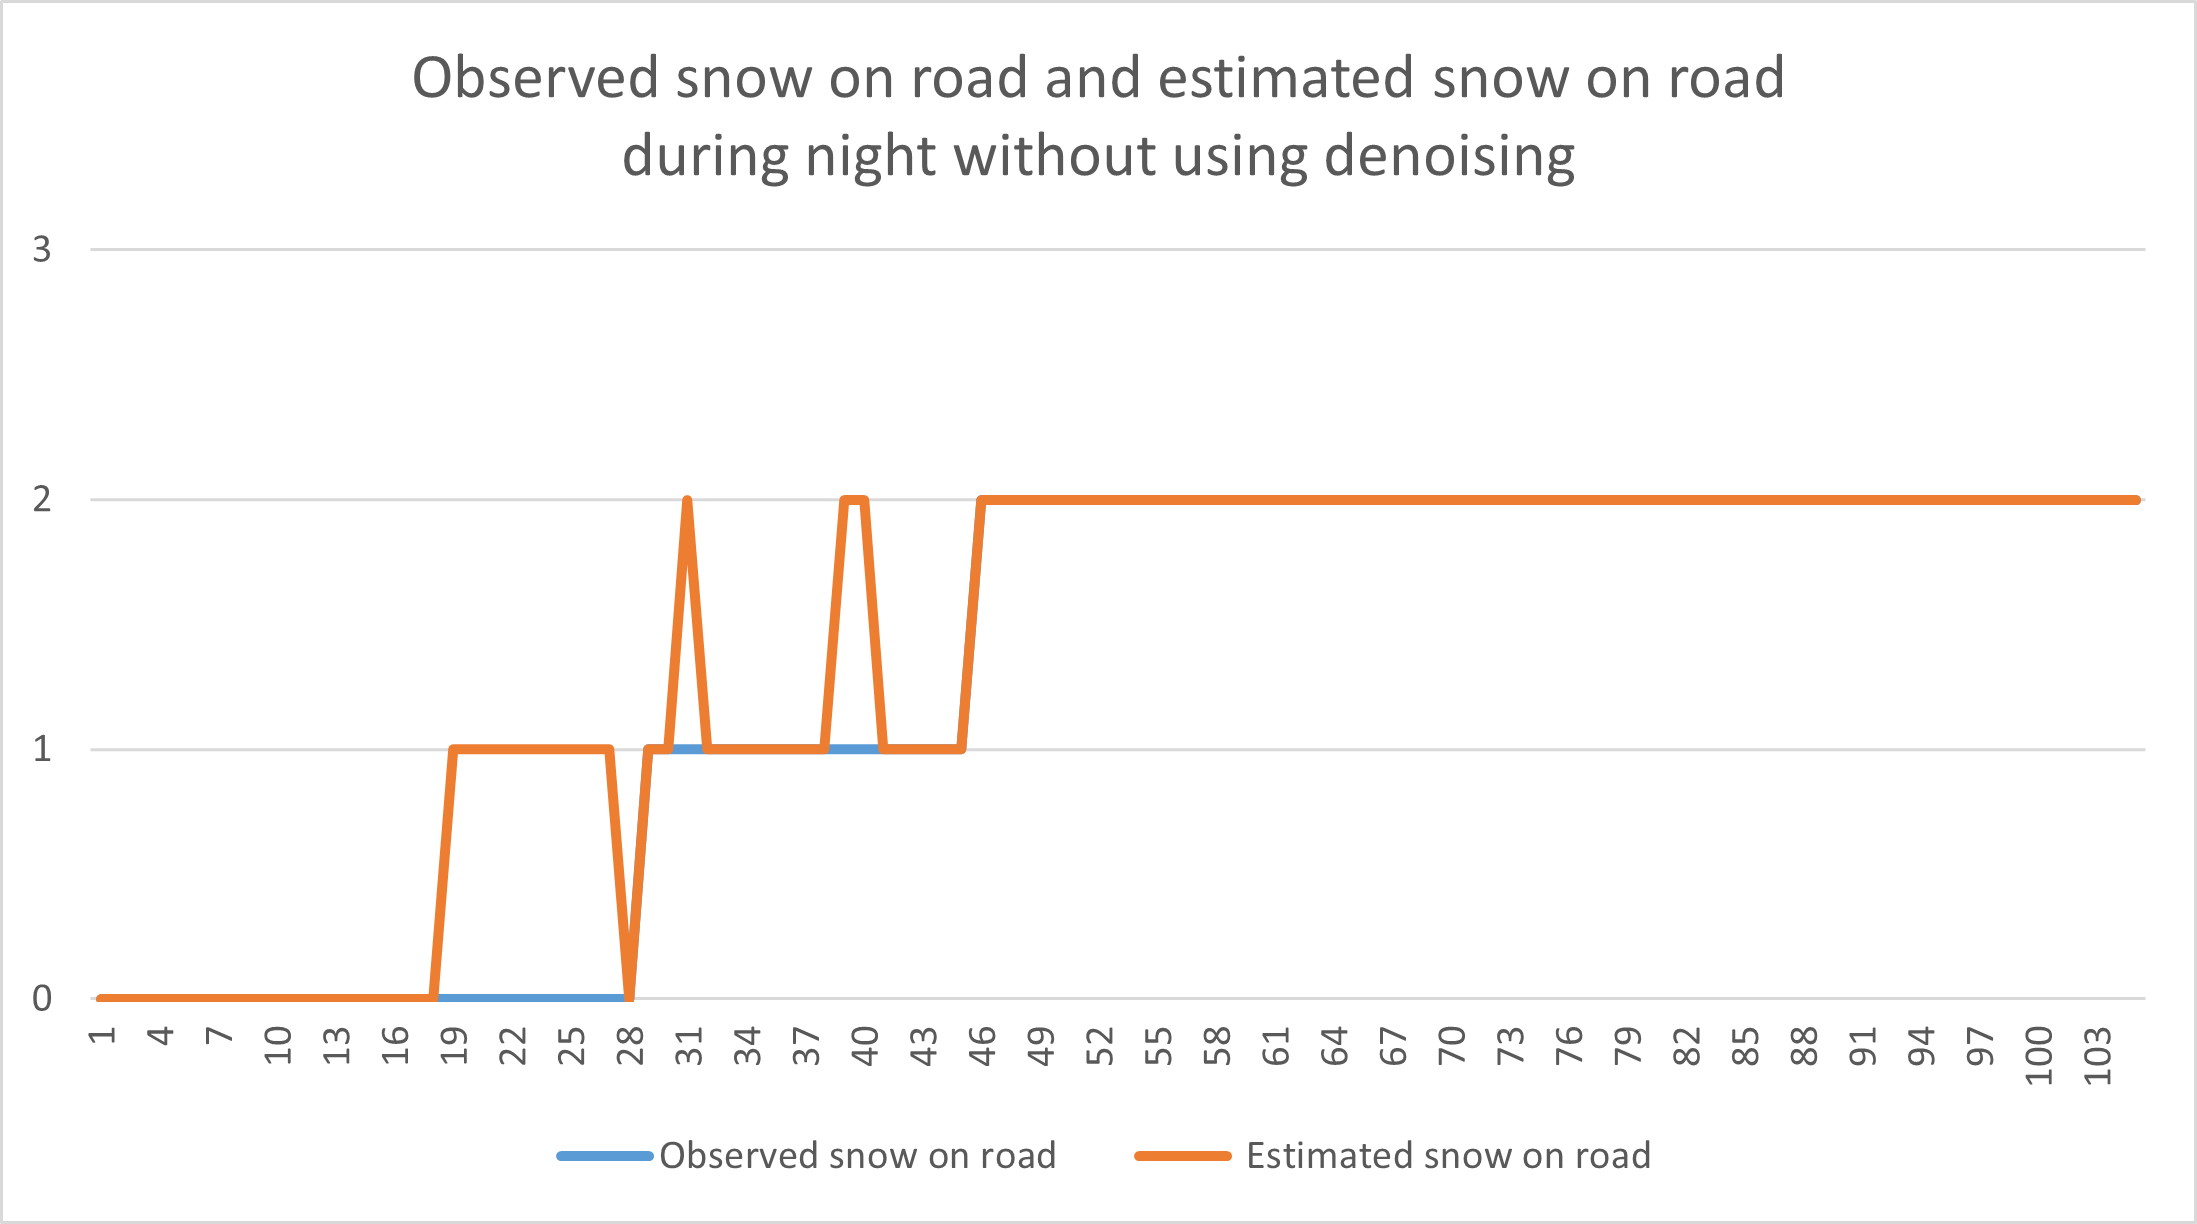
\includegraphics[width=\linewidth]{Images/computer_vision/snowOnRoad/nightResults_noise.png}
        \caption{Mesure durant la nuit, en bleu la valeur jugée à l'oeil, en orange la valeur interprétée}
        \label{fig:SnowOnRoad_noise_nightResults}
    \end{subfigure}
    \caption{Résultats de la mesure d'état de la route, sans suppression de bruit\emph{(échelle : 0 déneigée, 1 partiellement enneigée, 2 enneigée)}}
    \label{fig:SnowOnRoad_noise_results}
\end{figure}
Cette méthode a une précision de $90.8\%$ sur cet échantillon.\newpage

\subsubsection{Avec suppression de bruit}

\begin{figure}[H]
    \begin{subfigure}{.45\textwidth}
        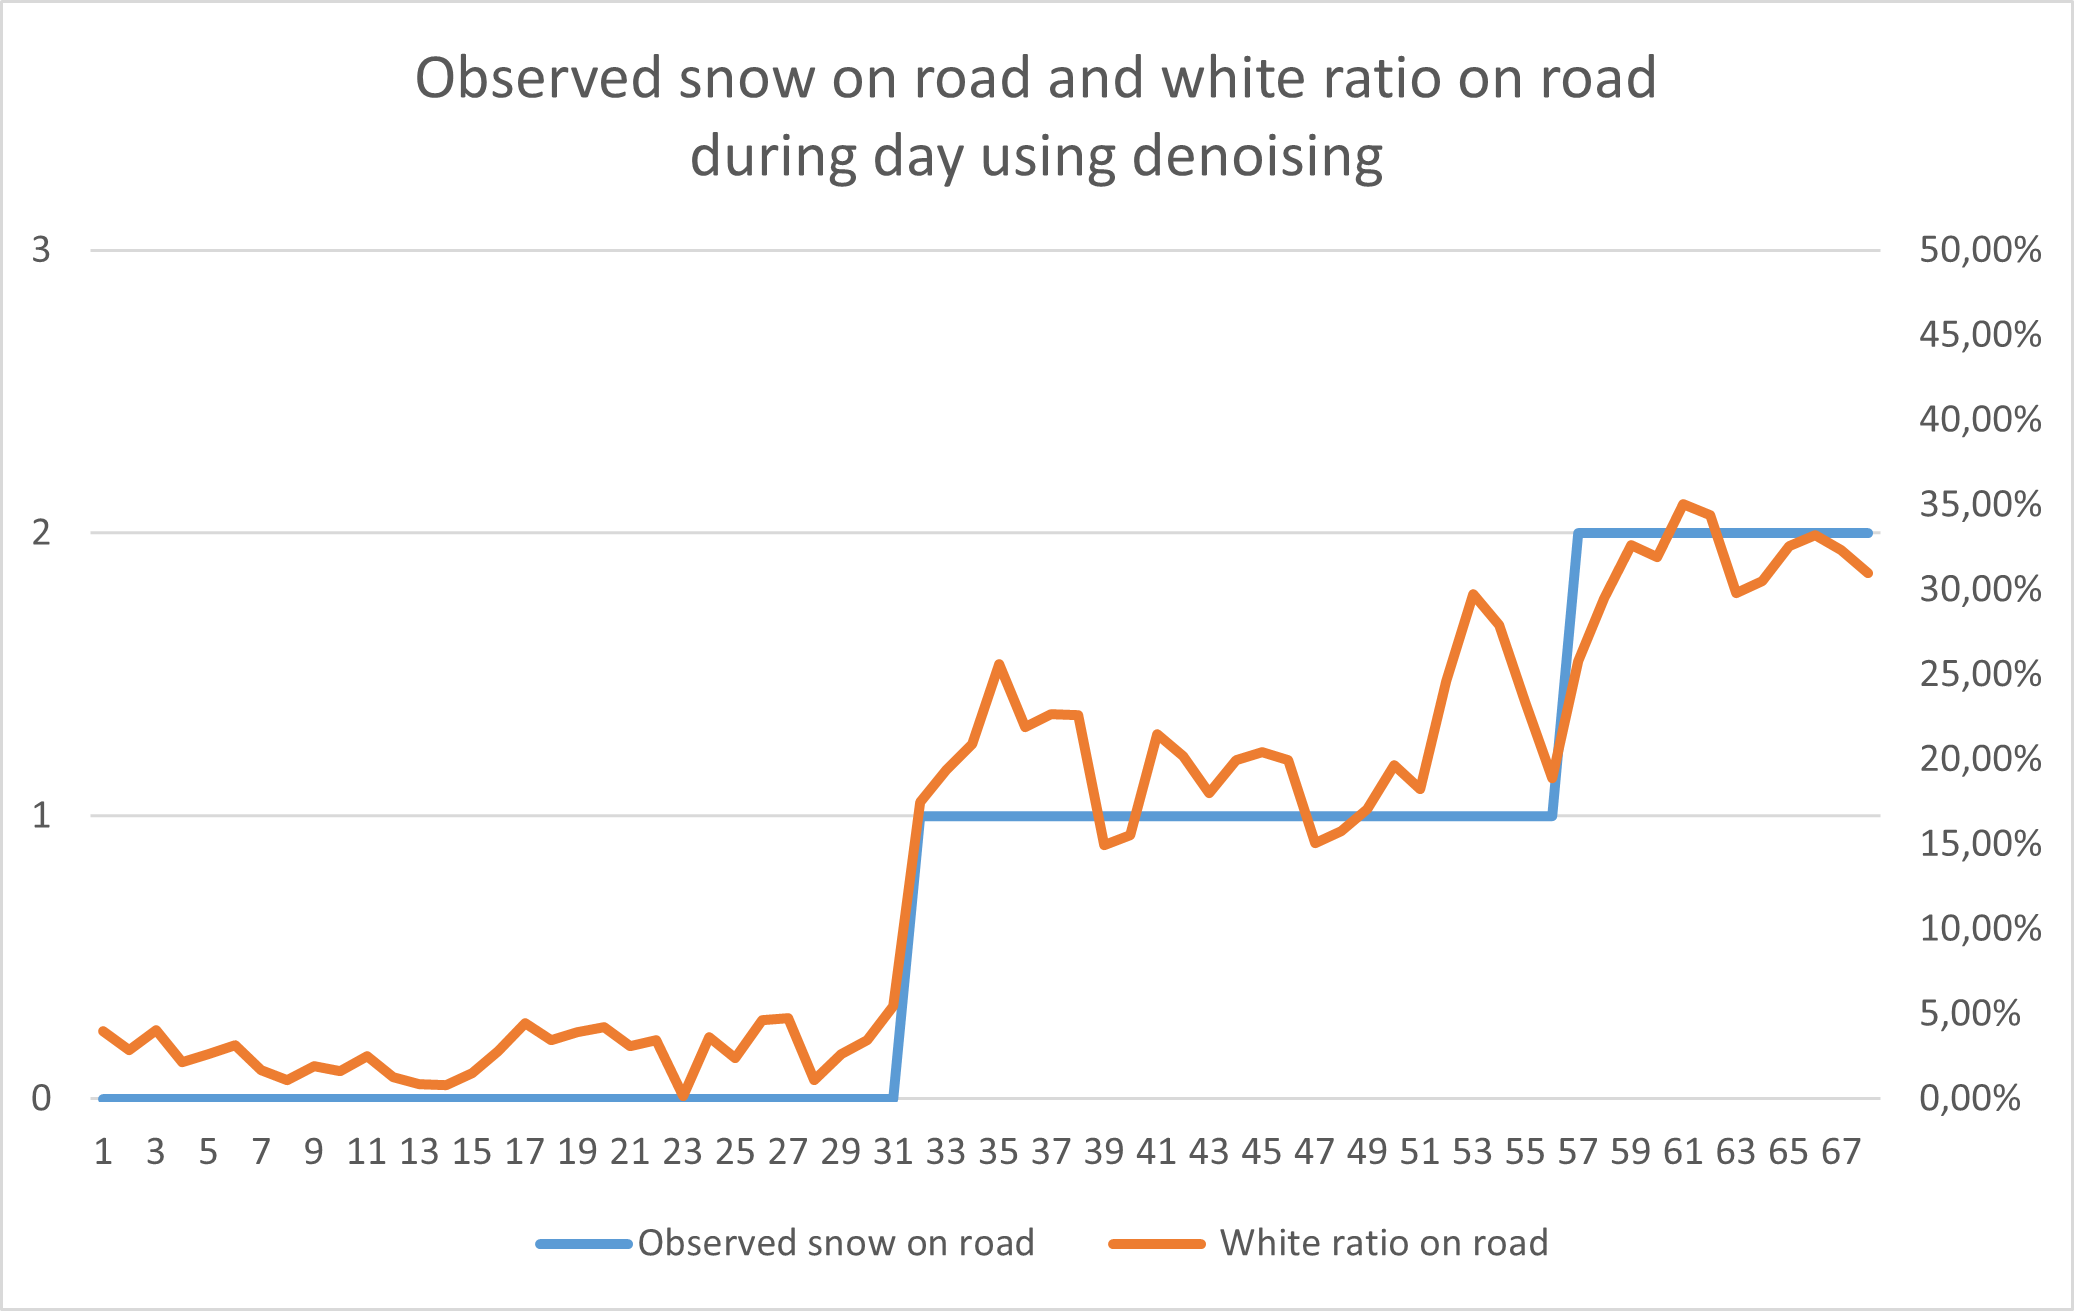
\includegraphics[width=\linewidth]{Images/computer_vision/snowOnRoad/dayMes_noNoise.png}
        \caption{Mesure durant la journée, en bleu la valeur jugée à l'oeil, en orange la valeur mesurée}
        \label{fig:SnowOnRoad_noNoise_dayMes}
    \end{subfigure}
    \hfill
    \begin{subfigure}{.45\textwidth}
        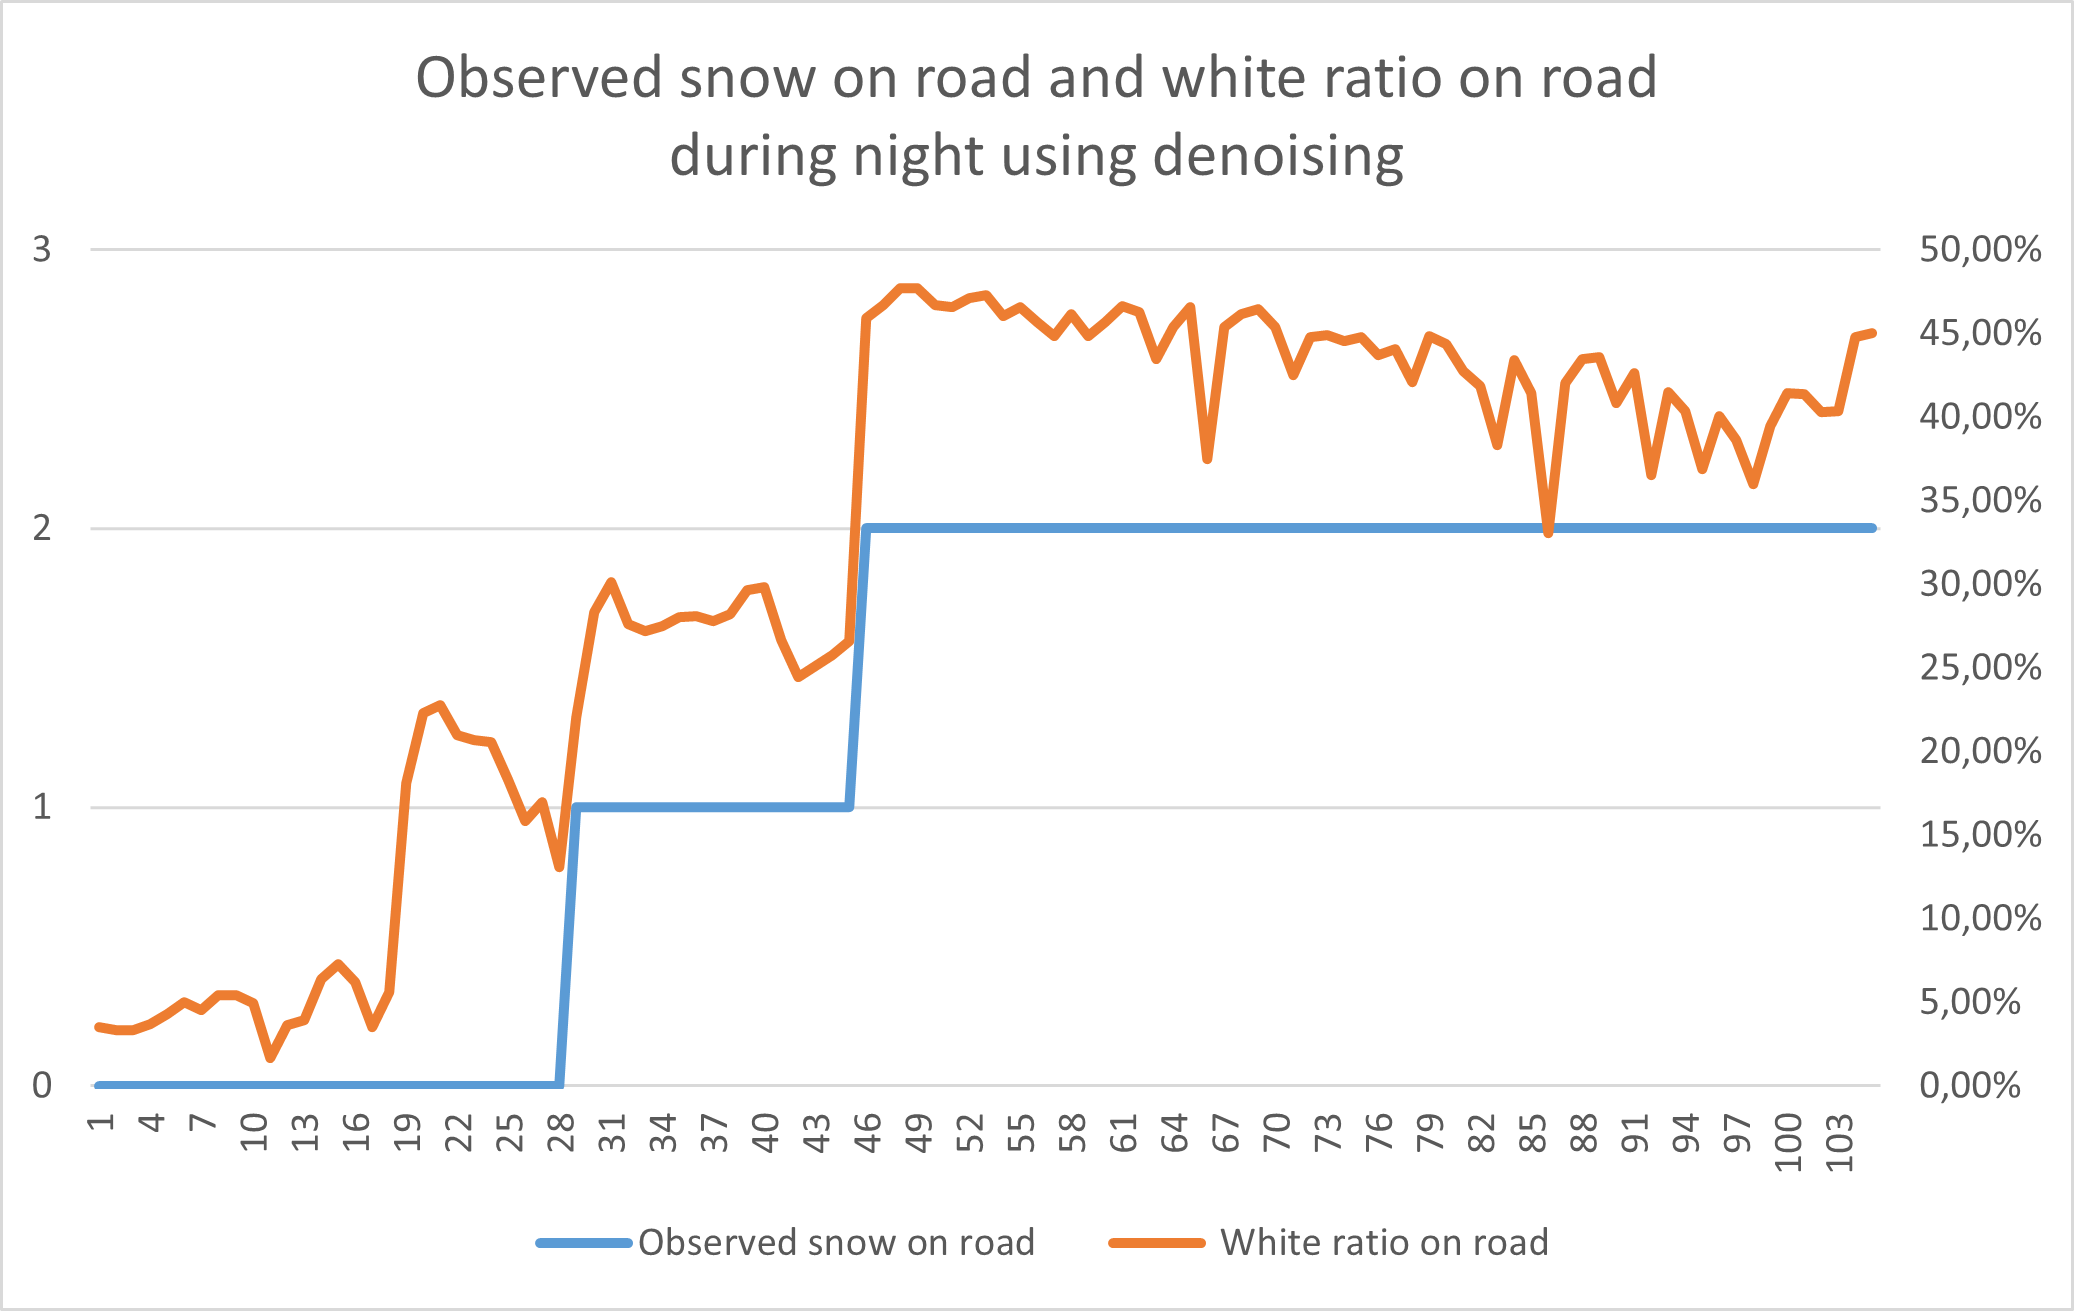
\includegraphics[width=\linewidth]{Images/computer_vision/snowOnRoad/nightMes_noNoise.png}
        \caption{Mesure durant la nuit, en bleu la valeur jugée à l'oeil, en orange la valeur mesurée}
        \label{fig:SnowOnRoad_noNoise_nightMes}
    \end{subfigure}
    \hfill
    \begin{subfigure}{.45\textwidth}
        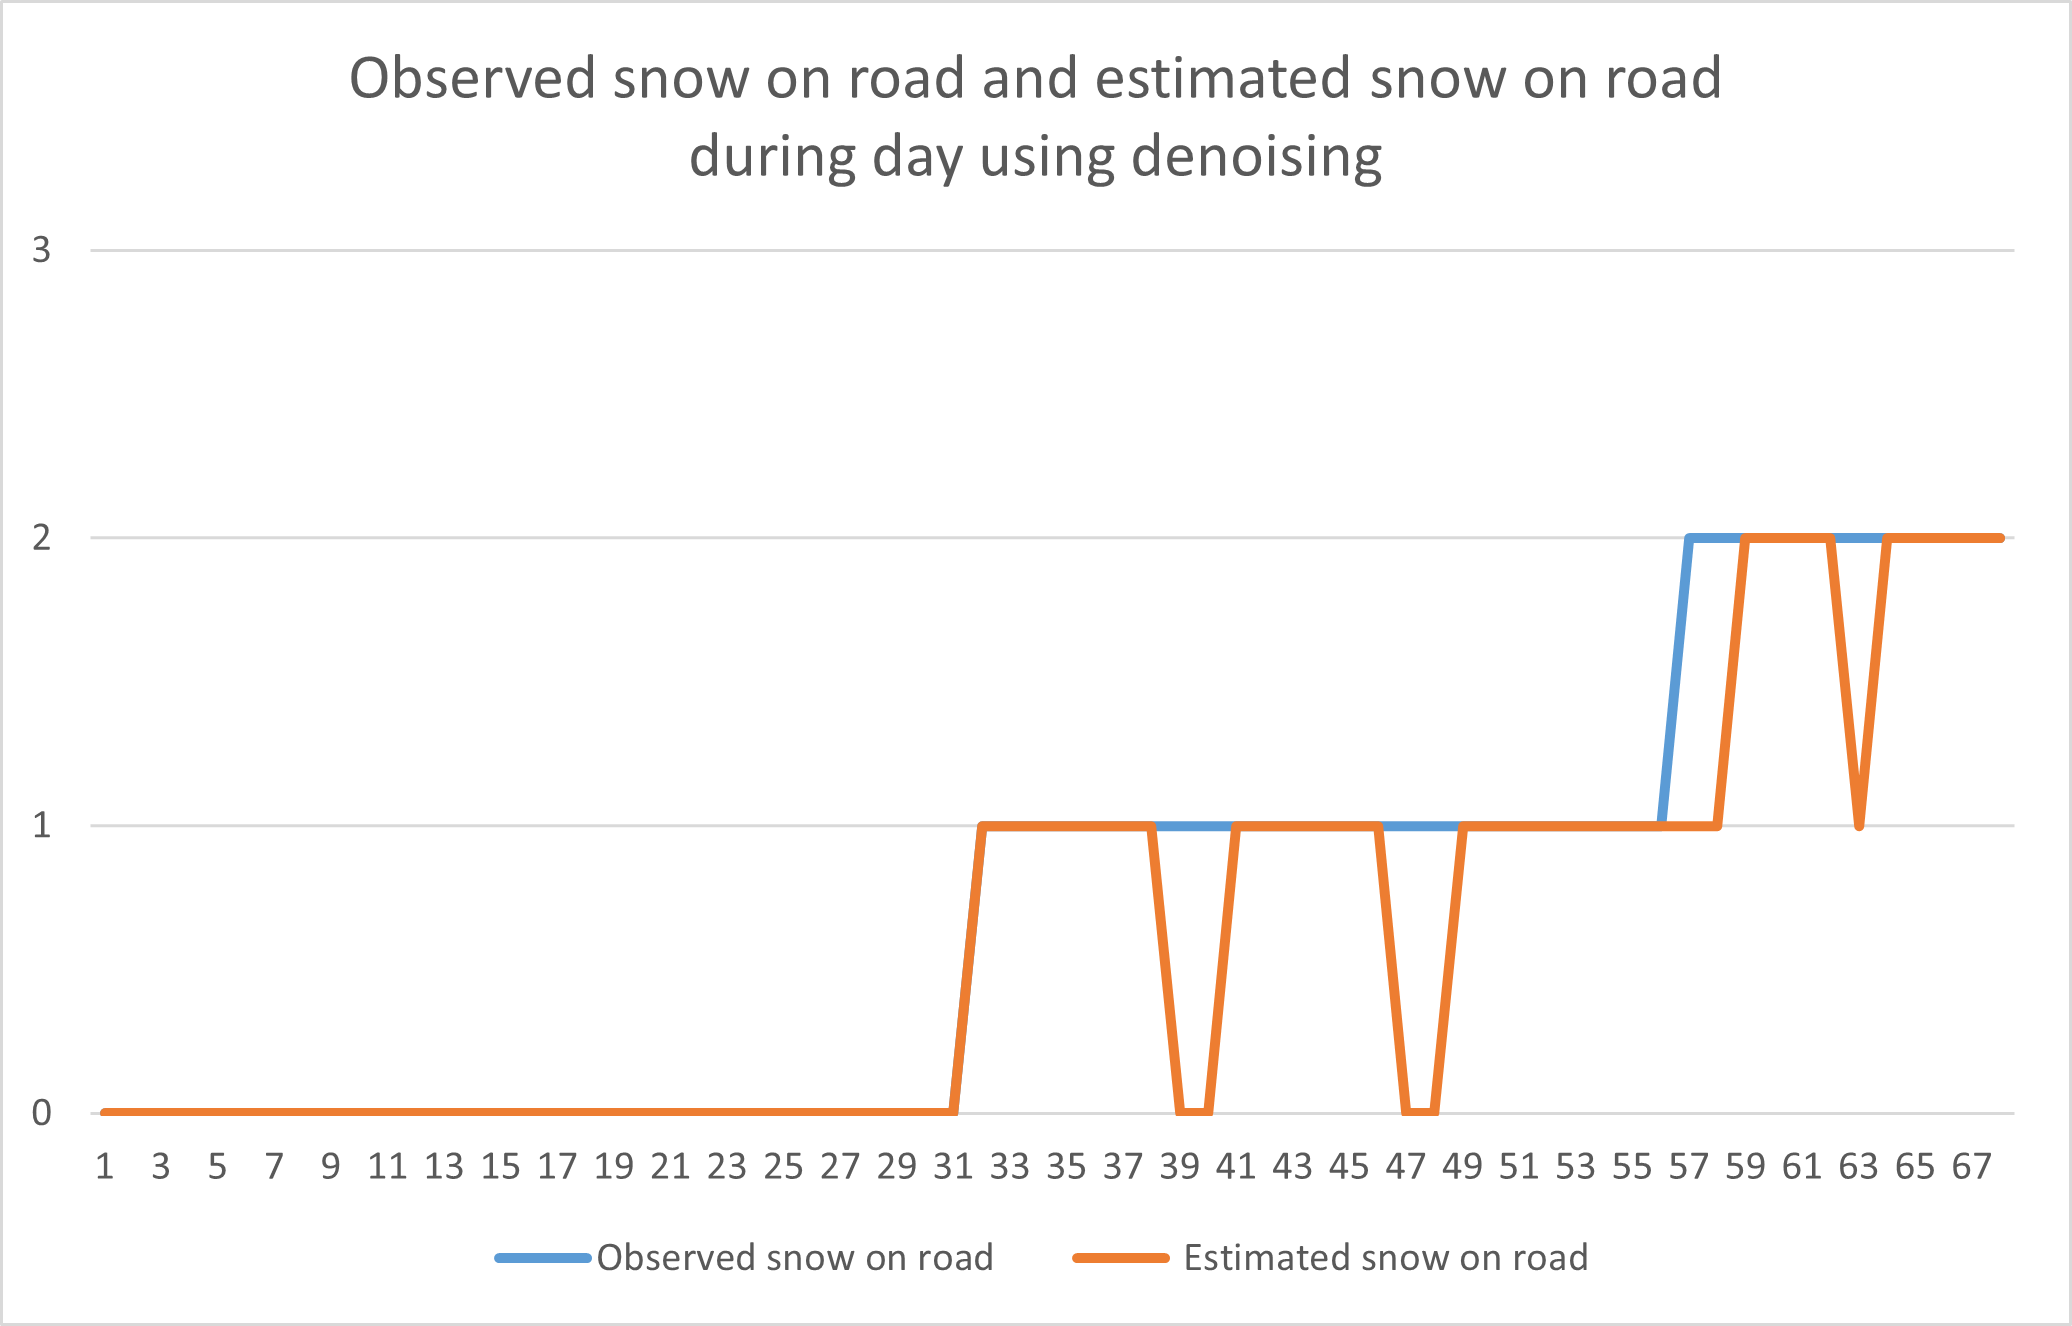
\includegraphics[width=\linewidth]{Images/computer_vision/snowOnRoad/dayResults_noNoise.png}
        \caption{Mesure durant la journée, en bleu la valeur jugée à l'oeil, en orange la valeur interprétée}
        \label{fig:SnowOnRoad_noNoise_dayResults}
    \end{subfigure}
    \hfill
    \begin{subfigure}{.45\textwidth}
        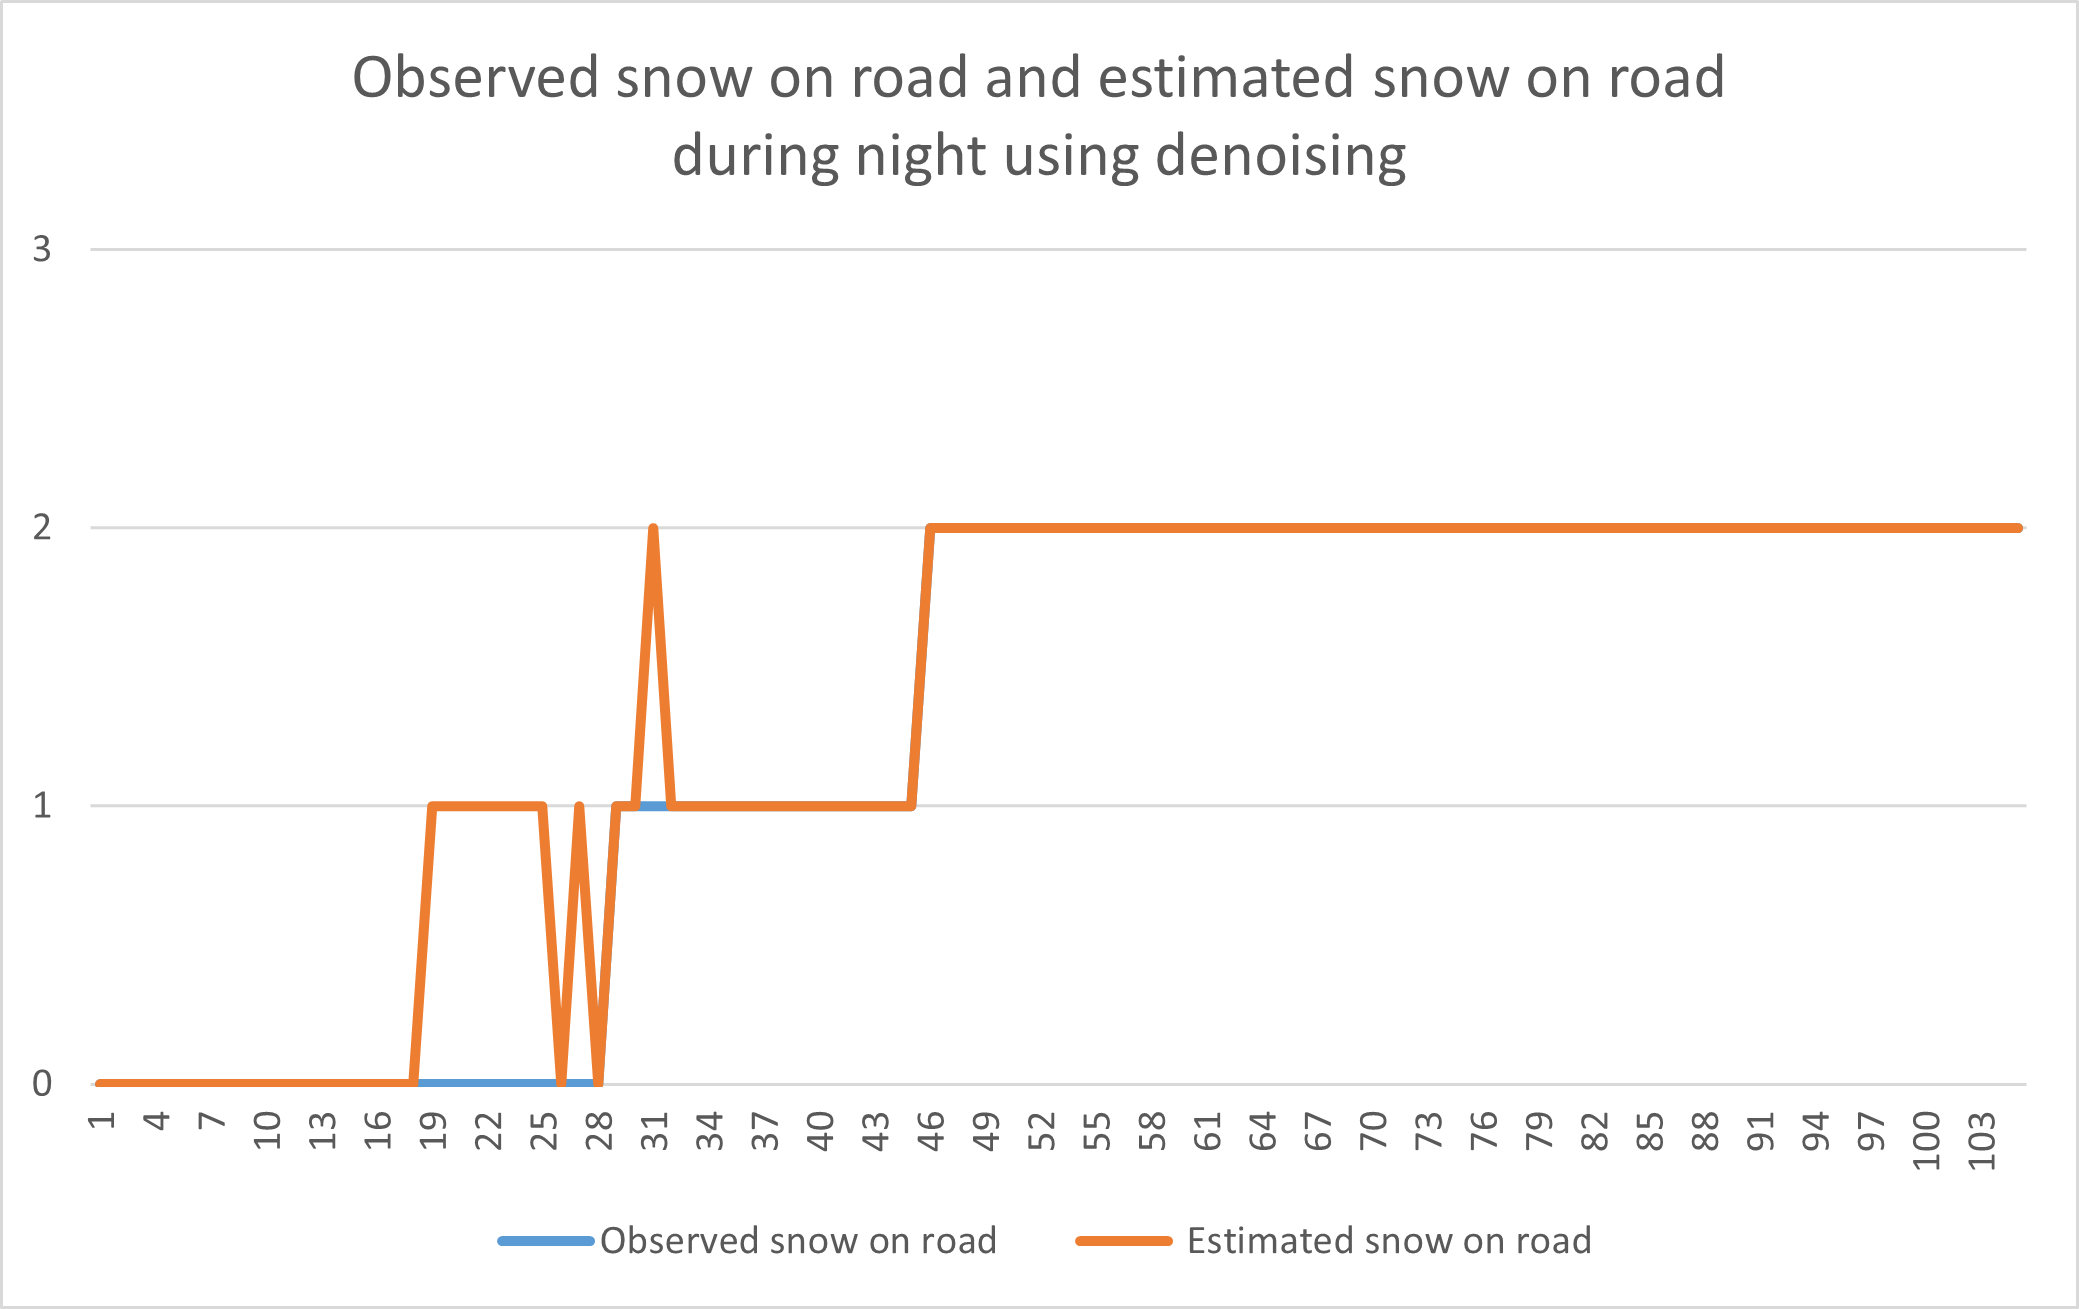
\includegraphics[width=\linewidth]{Images/computer_vision/snowOnRoad/nightResults_noNoise.png}
        \caption{Mesure durant la nuit, en bleu la valeur jugée à l'oeil, en orange la valeur interprétée}
        \label{fig:SnowOnRoad_noNoise_nightResults}
    \end{subfigure}
    \caption{Résultats de la mesure de débit de chute de neige, avec suppression de bruit\emph{(échelle : 0 déneigée, 1 partiellement enneigée, 2 enneigée)}}
    \label{fig:SnowOnRoad_noNoise_results}
\end{figure}
Cette méthode a également une précision de $90.8\%$ sur cet échantillon.


\subsubsection{Conclusion préliminaire}
Les deux méthodes ont un résultat identique sur cet échantillon. La méthode sans suppression de bruit est donc
retenue car elle demande moins de ressources.
On peut avoir l'impression que le système fonctionne moins de jour, mais cela est dû au fait que l'échantillon
représentant les routes enneigées était en fait des routes qu'on pourrait considérer \emph{entre} le degré 1 et 2.
Dans l'échantillon de nuit, les erreurs sont liées à des chasses-neige faussant la mesure avec leurs grands phares.
Une méthode évitant de mesurer lorsqu'un véhicule passe, comme cité au point \ref{snowfall} est nécessaire.\\
La méthode tel quel, fonctionne parfaitement.